\documentclass[11pt]{article}

% Change "review" to "final" to generate the camera-ready version.
\usepackage[review]{acl}

% Standard package includes
\usepackage{times}
\usepackage{latexsym}
\usepackage[T1]{fontenc}
\usepackage[utf8]{inputenc}
\usepackage{microtype}
\usepackage{inconsolata}
\usepackage{graphicx}
\usepackage{adjustbox}
\usepackage{subcaption}
\usepackage{caption}
\usepackage{placeins} % for \FloatBarrier

% Allow double-column floats (table*) to place more easily
\setcounter{dbltopnumber}{5}
\renewcommand{\dbltopfraction}{0.95}
\renewcommand{\dblfloatpagefraction}{0.95}
\usepackage[table]{xcolor}


% Paper-specific packages
\usepackage{amsmath,amssymb,amsthm}
\usepackage{booktabs}
\usepackage{multirow}
\usepackage{algorithm}
\usepackage{algorithmic}
\usepackage{xcolor}
\newcommand{\conv}[1]{#1\textsuperscript{\textdagger}}
\newcommand{\postconv}[1]{\textcolor{black!55}{#1}}


% Theorems
\newtheorem{definition}{Definition}
\newtheorem{lemma}{Lemma}
\newtheorem{proposition}{Proposition}

%\title{Active Learners are Efficient Rerankers}
\title{Active Learners as Efficient PRP Rerankers}

\begin{document}
\maketitle


%\begin{abstract}
%We study efficient LLM based reranking for Retrieval Augmented Generation (RAG) and argue that standard Pairwise Ranking Prompting (PRP) pipelines are ill-suited to LLM pairwise judgments. PRP methods typically plug LLM comparisons into classical sorting routines, but LLM preferences can depend on order and may violate transitivity, undermining the assumptions that sorting relies on and potentially increasing the number of LLM calls. We instead cast LLM reranking as active ranking under noisy pairwise comparisons and adopt algorithms designed for stochastic feedback. Across Information Retrieval (IR) benchmarks, these methods achieve competitive NDCG@10 with substantially fewer comparisons. To further reduce cost, we introduce a \emph{randomized direction oracle} that uses a single LLM call per comparison by uniformly randomizing prompt order, aligning the comparison process with the noisy active ranking setting. This oracle reduces LLM calls by about half relative to bidirectional PRP for both active and sorting based rankers, sometimes with a small drop in NDCG@10.
%\end{abstract}

% \begin{abstract}
% LLM pairwise ranking prompting (PRP) composes comparisons via classical sorting.
% This is mismatched to practice: LLM pairwise judgments are noisy, order-sensitive, and can be intransitive, while deployments care about top-$K$ quality under a call budget.
% We reframe reranking as active learning from noisy pairwise comparisons and benchmark active rankers as
% drop-in replacements for sorting-based PRP, improving NDCG@10 per call in the call-constrained regime.
% In addition, leveraging this noise-robust framing, we introduce a randomized-direction oracle that uses one
% LLM call per pair by randomizing prompt order and canonicalizing outcomes, inducing direction-consistent win
% probabilities despite order effects.
% \end{abstract}
%\begin{abstract}
%Pairwise Ranking Prompting (PRP) elicits pairwise preference judgments from LLMs, which are typically aggregated using classical sorting algorithms.
%This is mismatched to practice: LLM preferences are noisy, order-sensitive, and can be intransitive, while deployments care about top $K$ quality under a call budget. We reframe reranking as active learning from noisy pairwise comparisons and benchmark active rankers as
%drop-in replacements for PRP sorting algorithms, improving NDCG@10 per call in the call-constrained regime. Additionally, leveraging this noise-robust framework, we introduce a randomized-direction oracle that uses a single LLM call per pair by randomizing the prompt order, ensuring order consistency despite inherent call bias
%\end{abstract}

\begin{abstract} Pairwise Ranking Prompting (PRP) elicits pairwise preference judgments from LLMs, which are typically aggregated using classical sorting algorithms. This is mismatched to practice: LLM preferences are noisy, order-sensitive, and can be intransitive, while deployments care about top $K$ quality under a call budget. We reframe reranking as active learning from noisy pairwise comparisons and benchmark active rankers as drop-in replacements for PRP sorting algorithms, improving NDCG@10 per call in the call-constrained regime. Additionally, leveraging this noise-robust framework, we introduce a randomized-direction oracle that uses a single LLM call per pair by randomizing the prompt order, ensuring order consistency despite inherent call bias. \end{abstract}


% NO SE SI VALE LA PENA MENCIONAR AL MIXTO EN EL ABSTRACT, PERO LO DEJO ACA POR LAS DUDAS: We further introduce a \emph{mixture oracle} parameterized by $p\in[0,1]$ that interpolates between bidirectional and randomized direction oracles, enabling a tunable tradeoff between LLM call budget and comparison reliability. Respuesta (jere): para mi no vale la pena 


\section{Introduction}
LLMs are increasingly used as rerankers for retrieval-augmented generation (RAG): given a query and a candidate list,
a pairwise LLM judge selects an ordered top-$K$ subset for the context window, which can strongly affect downstream answer quality
\citep{zhu2023llmir,dong2024grag,sun2025dynamicrag}.
In practice, reranking is call-limited: LLM invocations dominate cost and latency, and the goal is a prefix (top-$K$), not a fully sorted list.

A common implementation of PRP treats pairwise LLM judgments as a comparator and invokes a sorting routine
\citep{qin2024pairwise,sun2023chatgptsearch}.
This ``LLM-as-comparator'' abstraction is convenient but structurally mismatched:
comparison-based sorting assumes stable, approximately transitive comparisons, while LLM judgments are stochastic, order-sensitive, and can violate transitivity.
As a result, sorting can waste budget polishing an unstable permutation rather than improving the top-$K$ that matters downstream.
Moreover, sorting optimizes a full permutation only at termination; under a strict call budget, it need not yield a strong top-$K$ prefix at intermediate budgets.

This gap is amplified by order effects: outcomes can depend on which passage is shown first
\citep{shi2024judges,yin2025fragile,jeong2025comparativetrap}.
To mitigate this, PRP often queries both prompt directions and aggregates, roughly doubling inference cost per compared pair
\citep{qin2024pairwise,wu2025realtimeprp}.
Yet even after bidirectional prompting, preference cycles can persist, so additional calls are often spent managing noise under a fixed budget.

We therefore reframe reranking as active learning from noisy pairwise comparisons rather than sorting:
each LLM call is a label query, and the system's question becomes which pairs to query to recover a strong top-$K$ within a budget.
This aligns reranking with active ranking / best-$K$ identification under noisy comparisons, where algorithms adaptively select informative pairs under stochastic feedback
\citep{mohajer2017active,heckel2016activeranking,shah2018simplerobust,ren2020bestk}.
Related PRP methods already hint at this view via adaptive pairing schedules \citep{luo-etal-2024-prp}.

Concretely, we ask whether replacing PRP-based sorting with active ranking yields practical efficiency gains in LLM reranking.
Since active rankers are designed to tolerate noisy pairwise feedback, our framing also enables a cheaper oracle:
we introduce a randomized-direction oracle that uses a single LLM call per pair by randomizing prompt order, yielding direction-consistent win probabilities despite order sensitivity.
On TREC DL2019/2020 with Flan-T5-XL, Mohajer with randomized-direction reaches 68.18 NDCG@10 by $B{=}200$ calls,
while the best sorting baseline matches this quality only at substantially larger budgets ($B{=}350$--$400$).


%\section{Introduction}

%Large language models (LLMs) are increasingly used as rerankers: given a query and
%a ranked candidate list from a first-stage retriever, an LLM judge is asked to
%decide which passages are more relevant, and the resulting ordering determines
%the evidence included in the RAG context window---a choice that can critically
%shape downstream answer quality
%\citep{zhou2025large, %zhu2023llmir,dong2024grag,sun2025dynamicrag}.
%The practical significance of reranking is reflected in rapid commercial
%adoption, with major cloud platforms offering reranking as a core capability.
%In this setting, LLM inference calls---not CPU-level operations---dominate
%latency and cost, and the objective is typically top-$K$ selection for
%context construction rather than computing a full total order.

%A common approach is to use an LLM as a pairwise judge. Pairwise Ranking
%Prompting (PRP) compares two candidate passages at a time and produces a full
%ranking by composing many such judgments, often by plugging the LLM comparator
%into a classical comparison-based sorting routine \citep{qin2024pairwise,sun2023chatgptsearch}. This “LLM-as-comparator” abstraction is convenient, but it inherits a mismatch: comparison-based sorting is designed to recover a single consistent total order using a comparator whose outcomes are stable and effectively transitive.

%Treating PRP as sorting introduces a deeper modeling mismatch:
%LLM pairwise judgments are often contextual and stochastic.
%In particular, outcomes can depend on which passage is presented first
%(direction sensitivity), a widely observed effect in LLM-as-a-judge settings
%\citep{shi2024judges,yin2025fragile,jeong2025comparativetrap}.
%To mitigate this, practitioners frequently query both prompt directions and
%aggregate, roughly doubling inference cost per compared pair
%\citep{qin2024pairwise,wu2025realtimeprp}.
%Moreover, even after controlling for direction effects, pairwise preferences
%can exhibit intransitivity, so the
%notion of a single ``sorted'' order may be ill-posed: the produced ranking can
%depend on the sequence of comparisons and additional calls may be spent
%resolving contradictions.

%Given this considerations, in this paper we suggest reframing reranking as an active learning
%problem with noisy comparisons rather than a sorting problem. Each LLM comparison is a label
%query revealing noisy pairwise preference information, and the central systems
%question becomes: \emph{which pairs should we query under a call budget to
%recover a high-quality top-$K$}? This aligns reranking with active ranking /
%top-$K$ identification from noisy pairwise comparisons, where algorithms are
%explicitly designed to adaptively select informative comparisons under
%stochastic feedback \citep{mohajer2017active,heckel2016activeranking,shah2018simplerobust,ren2020bestk}.
%Notably, some strong PRP methods already contain adaptive comparison schedules
%that resemble this view. For example, PRP-Graph uses Swiss-system-inspired
%pairings based on evolving standings, implicitly allocating comparisons to
%harder decisions \citep{luo-etal-2024-prp}.

%Here we ask whether replacing sorting-based PRP with active ranking algorithms yields
%practical efficiency gains in LLM reranking.
%First, we benchmark active ranking methods as drop-in alternatives to
%sorting-based PRP and find that they can achieve competitive NDCG@10 with
%substantially fewer pairwise judgments.
%Second, because active ranking theory naturally models \emph{noisy} pairwise
%feedback, we leverage this robustness to reduce \emph{per-pair} prompting cost:
%we introduce a \emph{randomized-direction oracle} that makes a single LLM call
%per pair by uniformly randomizing prompt order and canonicalizing the outcome,
%yielding direction-consistent pairwise win probabilities despite order
%sensitivity.
%Third, we evaluate this oracle both within active ranking algorithms and as a
%drop-in replacement inside classical sorting pipelines, quantifying the
%NDCG@10--cost trade-off under a call-centric accounting.

%Overall, our findings suggest that LLM-based reranking is best treated as
%budgeted learning from noisy comparisons rather than deterministic sorting:
%active rankers concentrate calls on informative pairs, and a randomized-direction
%oracle further reduces cost by requiring only one call per comparison while
%remaining direction-consistent.



%Large language models (LLMs) are increasingly being used as rankers to score and order a finite set of candidate documents or passages for a given query.
%The resulting decisions about what to retain---and how to order it---can
%strongly affect downstream quality. Retrieval-augmented generation (RAG) is a
%particularly important instance of this setting: a retriever produces a
%high-recall pool of passages, and reranking converts it into high-precision
%context selection by placing the most relevant evidence near the top, which
%directly impacts answer quality \citep{zhu2023llmir,dong2024grag,sun2025dynamicrag}.


%A common approach is to use an LLM as a pairwise judge. Pairwise Ranking
%Prompting (PRP) compares two candidate passages at a time and produces a full
%ranking by composing many such judgments, often within a classical sorting
%routine \citep{qin2024pairwise,sun2023chatgptsearch}. However, treating an LLM
%as a comparison oracle introduces practical and theoretical friction:
%\begin{itemize}
%  \item \textbf{Order sensitivity:} outcomes can depend on which passage is
%  presented first, a well-documented effect in LLM-as-a-judge settings
%  \citep{shi2024judges,yin2025fragile,jeong2025comparativetrap}.
%  \item \textbf{Cost and latency:} each pairwise judgment requires at least one
%  LLM call, and to mitigate order effects practitioners often query both prompt
%directions for every pair, roughly doubling inference cost
%  \citep{qin2024pairwise,wu2025realtimeprp}.
%\item \textbf{Intransitivity:} even when order effects are controlled, LLM
%  comparisons can exhibit preference cycles (e.g., $A \succ B$, $B \succ C$,
%  $C \succ A$), violating the consistent-comparator assumptions that
%  comparison-based sorting relies on. In such regimes, the produced ranking can
%  depend on the sequence of comparisons and may require redundant queries to
%  resolve contradictions.
%\end{itemize}


%These issues suggest reframing: rather than using LLM comparisons solely as a
%subroutine inside a sorting pipeline, we view reranking as an \emph{active
%ranking} problem over noisy pairwise preferences, where the system adaptively
%chooses which document pairs to compare in order to recover a high-quality
%top-$K$ list with fewer judgments \citep{mohajer2017active}. Several PRP methods
%already contain adaptive comparison scheduling that aligns with this view, even
%if not described in those terms. For example, PRP-Graph draws inspiration from
%Swiss-system tournaments---pairing candidates by current standings across rounds
%when constructing a ranking graph---and reports strong reranking performance
%with acceptable efficiency \citep{luo-etal-2024-prp}.

%\paragraph{Approach overview.}
%We first ask whether replacing sorting-based PRP with active ranking algorithms
%yields practical efficiency gains in LLM reranking; empirically, we observe
%substantial reductions in pairwise judgments while maintaining competitive
%NDCG@10. Second, because active ranking methods are designed to tolerate noisy
%pairwise feedback, we leverage this robustness to reduce per-pair prompting
%cost: we introduce a \emph{randomized direction oracle} that makes a single LLM
%call per pair by randomly choosing the prompt order and mapping the output to a
%canonical direction, replacing bidirectional PRP (two calls per pair) with a
%stochastic but well-defined comparison model. Third, we evaluate this oracle
%first within active ranking algorithms and then as a drop-in replacement inside
%classical comparison-based sorting pipelines, quantifying the trade-off between
%NDCG@10 and total LLM call budget.

%\paragraph{Contributions.}
%\begin{enumerate}
%  \item We benchmark active ranking methods for LLM reranking and show they
%  achieve competitive NDCG@10 with substantially fewer LLM pairwise calls than
%  sorting-based PRP.

%  \item We introduce a \emph{randomized direction oracle} that uses one LLM call
%  per pair (instead of two-direction PRP) and yields direction-consistent
%  pairwise win probabilities.

%  \item We empirically study the effect of stochastic comparisons on reranking:
%  active ranking methods are more robust to the single-call oracle and deliver a
%  better NDCG@10--cost trade-off than comparator-based sorting; when used as a
%  drop-in comparator for sorting-based PRP, the oracle reduces calls by up to
%  50\% in some pipelines with only a small NDCG@10 drop.
%\end{enumerate}

\section{Related Work}

\noindent\textbf{Pairwise LLM reranking (PRP).}
Pairwise Ranking Prompting (PRP) sorting procedures use an LLM comparator and compose pairwise judgments into a ranking \citep{sun2023chatgptsearch,qin2024pairwise}.
Most pipelines plug the PRP unit as a comparator into classical sorting, targeting a full order rather than a top-$K$ prefix under a call budget.
This creates a structural mismatch. Because LLM comparisons are noisy and can be intransitive, extra comparisons may refine an ill-posed global order rather than improve the prefix.

\noindent\textbf{Order effects and bidirectional prompting.}
LLM comparisons can be direction-sensitive \citep{shi2024judges,yin2025fragile,jeong2025comparativetrap}, so PRP often queries both prompt orders, roughly doubling cost \citep{qin2024pairwise,wu2025realtimeprp}.
We instead leverage a noise-robust framing to define a randomized-direction oracle that uses one call per pair by randomizing comparison order, inducing direction-independent win probabilities, despite order sensitivity.

\noindent\textbf{Beyond sorting: graphs, tournaments, and active ranking.}
Some PRP variants depart from sorting, e.g., PRP-Graph aggregates a weighted comparison graph and uses adaptive pairings (Swiss-style scheduling) \citep{luo-etal-2024-prp}; tournament-style designs similarly structure comparisons for efficiency \citep{chen2024tourrank}. Our work makes this scheduling question explicit by reframing reranking as active learning from noisy pairwise comparisons and evaluating active top-$K$ identification methods as drop-in replacements for PRP-based sorting \citep{heckel2016activeranking,shah2018simplerobust,ren2020bestk,mohajer2017active}.

\noindent\textbf{Orthogonal efficiency.}
Other work reduces cost by changing the prompting primitive (setwise/listwise) or allocating inference by uncertainty \citep{zhuang2024setwise,huang2025tssetrank,wang2025realm}.
Our focus is orthogonal: for pairwise ranking, we study (i) noise-aware comparison scheduling (active ranking) and (ii) a cheaper single-call oracle.


%\section{Related Work}

%\noindent\textbf{LLM reranking with pairwise prompting (PRP).}
%Pairwise ranking prompting (PRP) is a common and effective design point for LLM-based reranking
%\citep{sun2023chatgptsearch,qin2024pairwise}.
%However, standard PRP pipelines compose LLM comparisons via classical sorting routines,
%implicitly assuming a stable (approximately transitive) comparator
%\citep{qin2024pairwise,sun2023chatgptsearch,wisznia2025batchingcaching},
%while LLM judgments can be order-sensitive and noisy
%\citep{shi2024judges,yin2025fragile,jeong2025comparativetrap}.
%Our work targets this mismatch by (i) replacing sorting with budgeted active top-$K$ identification under noisy comparisons
%\citep{heckel2016activeranking,shah2018simplerobust,ren2020bestk,mohajer2017active}
%and (ii) introducing a single-call randomized-direction oracle that remains well-posed under order effects.

%\noindent\textbf{Composing PRP comparisons: sorting, graphs, and tournaments.}
%Most PRP systems aggregate pairwise LLM judgments via sorting (e.g., heapsort), effectively treating the LLM as a deterministic comparator
%\citep{qin2024pairwise,sun2023chatgptsearch}.
%PRP-Graph departs from pure sorting by constructing a weighted comparison graph and aggregating it into a final ranking
%\citep{luo-etal-2024-prp};
%notably, its Swiss-system-inspired pairing schedule already suggests that \emph{which} pairs are queried can matter as much as \emph{how} outcomes are aggregated.
%Tournament-style strategies similarly structure comparisons to improve efficiency and parallelism \citep{chen2024tourrank}.
%We make this scheduling question explicit by evaluating active comparison-selection algorithms as drop-in alternatives to sorting-based PRP under the same pairwise oracle interface.

%\noindent\textbf{Active ranking and top-$K$ identification from noisy comparisons.}
%Our framing connects reranking to active ranking and best-$K$ identification under stochastic pairwise feedback, where algorithms and query-complexity analyses are designed for noisy outcomes and do not require global transitivity
%\citep{heckel2016activeranking,shah2018simplerobust,ren2020bestk,mohajer2017active}.
%This perspective matches two practical realities of LLM reranking: (i) the deployment objective is typically a high-quality top-$K$ set/list rather than a full total order, and (ii) LLM pairwise judgments can be stochastic and context-dependent.
%We operationalize this connection by benchmarking active ranking methods under a call-centric budget and comparing them directly to classic PRP sorting and PRP-Graph.



%\noindent\textbf{Changing the prompting primitive: setwise and uncertainty-aware rerankers.}
%A complementary line of work reduces cost by changing the oracle itself:
%setwise prompting compares small subsets per call \citep{zhuang2024setwise},
%and adaptive variants allocate inference based on uncertainty or variability in judgments \citep{huang2025tssetrank,wang2025realm}.
%These methods are strong alternatives. Our focus is orthogonal: we study what efficiency gains are achievable \emph{without} leaving the pairwise-PRP setting, so existing PRP infrastructure and caching interfaces remain applicable.

%\noindent\textbf{Order effects and reliability of LLM judgments.}
%Presentation-order effects and other biases are widely observed in LLM-as-a-judge settings, raising concerns about comparator stability and reproducibility
%\citep{ye2024calm_suchas,survey_llm_judge,shi2024judges,yin2025fragile,jeong2025comparativetrap}.
%A common mitigation in PRP is to query both prompt directions and aggregate, which roughly doubles inference cost per compared pair
%\citep{qin2024pairwise,wu2025realtimeprp}.
%We instead define a randomized-direction oracle that induces a direction-consistent comparison probability with a single LLM call per pair, aligning the oracle with the noisy-comparison assumptions used by active ranking while directly targeting call efficiency.

%\noindent\textbf{Call-centric cost models for PRP.}
%Recent work argues PRP efficiency should be analyzed in terms of LLM inference calls, and that batching/caching can change which composition routines are cost-optimal \citep{wisznia2025batchingcaching}.
%We adopt this call-centric view and report unique-pair counts to make caching effects explicit, enabling apples-to-apples comparisons across composition and scheduling strategies.



%\section{Related Work}

%\paragraph{LLMs for ranking and reranking.}
%LLMs have been used as rerankers in pointwise, pairwise, and listwise prompting regimes \citep{sun2023chatgptsearch,qin2024pairwise,zhu2023llmir}. Pairwise reranking is effective but can be costly, motivating practical efficiency optimizations \citep{wu2025realtimeprp}. Most pairwise PRP pipelines still compose comparisons via classical sorting routines; we instead focus on comparison \emph{scheduling} and aggregation when comparisons are noisy and calls are the bottleneck.

%\paragraph{Composition strategies for pairwise PRP: graphs and tournaments.}
%Beyond sorting-based composition, PRP-Graph constructs a weighted comparison graph and then aggregates it into a final ranking \citep{luo-etal-2024-prp}. Notably, PRP-Graph already contains an \emph{adaptive} comparison schedule: its Swiss-system-inspired pairings depend on evolving standings, implicitly allocating comparisons to harder decisions. We view this as evidence that adaptive pairing is beneficial even when not framed explicitly as active learning; our work studies this idea through the lens of active ranking algorithms with comparison/sample-complexity guarantees \citep{heckel2016activeranking,shah2018simplerobust,falahatgar2018limits,ren2020bestk,mohajer2015noisy}. Tournament-style strategies similarly structure comparisons to improve efficiency and parallelization \citep{chen2024tourrank}.

%\paragraph{Changing the prompting primitive: setwise and uncertainty-aware rerankers.}
%A complementary line of work reduces cost by changing the oracle itself. Setwise prompting compares small subsets per call \citep{zhuang2024setwise}, and adaptive variants allocate a fixed inference budget based on uncertainty or variability in LLM judgments \citep{huang2025tssetrank}. Uncertainty-aware approaches such as REALM explicitly model uncertainty and refine rankings via recursive updates \citep{wang2025realm}. These methods are strong alternatives; our focus is on what can be gained \emph{without} changing the pairwise PRP primitive.

%\paragraph{Prompt-direction sensitivity in LLM comparisons.}
%Presentation-order effects are widely observed in LLM-as-a-judge settings \citep{shi2024judges,yin2025fragile}, and pairwise comparisons can amplify superficial preferences \citep{jeong2025comparativetrap}. This motivates careful comparator design and aggregation procedures that remain effective under directional bias and inconsistencies.

%\paragraph{LLM-centric cost models for PRP.}
%Recent work argues PRP efficiency should be analyzed in terms of \emph{inference calls}, and that batching and caching can change which composition routines are cost-optimal \citep{wisznia2025batchingcaching}. We adopt this call-centric view and report unique-pair counts to make caching effects explicit.


% Preamble (make sure this is defined somewhere before the table)

\begin{table*}[t]
\centering
\begin{adjustbox}{max width=\textwidth}
\scriptsize
\begin{tabular}{c l rrrrrrrrr}
\toprule
& & \multicolumn{9}{c}{Number of comparisons (budget)} \\
\cmidrule(lr){3-11}
Oracle & Ranker & 100 & 150 & 200 & 250 & 300 & 350 & 400 & 450 & 500 \\
\midrule

\multirow{6}{*}{\rotatebox[origin=c]{90}{Bidirectional}}
& BubbleSort        & \underline{49.27} & \underline{49.27} & \underline{56.43} & \underline{56.43} & 56.42 & 56.98 & 60.25 & 60.30 & 60.51 \\
& HeapSort          & 6.81 & 6.13 & 6.13 & 9.28 & 23.04 & 41.84 & 54.29 & 62.81 & \textbf{68.21} \\
& QuickSort         & \textbf{55.93} & \textbf{55.89} & 55.87 & 56.20 & 56.20 & 56.20 & 56.40 & 56.59 & 56.68 \\
& PAC + Bubble      & \underline{49.27} & \underline{49.27} & 49.27 & 49.27 & \underline{57.52} & \underline{60.59} &
\conv{60.61} & \postconv{60.61} & \postconv{60.61} \\
& Mohajer + Bubble  & 30.12 & 30.12 & \textbf{62.34} & \textbf{64.80} & \textbf{66.09} & \textbf{66.28} & \textbf{66.83} &
\conv{\textbf{67.02}} & \postconv{\underline{67.02}} \\
& Mohajer           & 30.12 & 30.12 & \textbf{62.34} & \textbf{64.80} & \textbf{66.09} & \textbf{66.28} & \underline{66.81} &
\conv{\underline{66.96}} & \postconv{66.96} \\

\midrule

\multirow{6}{*}{\rotatebox[origin=c]{90}{Randomized}}
& BubbleSort        & \underline{55.57} & 56.10 & 59.40 & 59.39 & 61.64 & 62.15 & 63.81 & 64.37 & 65.80 \\
& HeapSort          & 6.85 & 16.42 & 50.32 & 65.41 & \underline{67.90} & \underline{68.33} & \textbf{68.54} & \textbf{68.27} & \textbf{68.71} \\
& QuickSort         & 53.92 & 55.42 & 55.66 & 57.28 & 57.29 & 58.75 & 60.12 & 62.29 & 63.14 \\
& PAC + Bubble      & 49.27 & \underline{56.81} &
\conv{\underline{59.78}} & \postconv{59.78} & \postconv{59.78} & \postconv{59.78} & \postconv{59.78} & \postconv{59.78} & \postconv{59.78} \\
& Mohajer + Bubble  & \textbf{60.68} & \textbf{66.42} & \textbf{68.18} & \underline{67.80} & 67.79 & \textbf{68.39} &
\conv{67.89} & \postconv{67.89} & \postconv{67.89} \\
& Mohajer           & \textbf{60.68} & \textbf{66.42} &
\conv{\textbf{68.18}} & \postconv{\textbf{68.18}} & \postconv{\textbf{68.18}} &
\postconv{68.18} & \postconv{\underline{68.18}} & \postconv{\underline{68.18}} & \postconv{\underline{68.18}} \\

\bottomrule
\end{tabular}%
\end{adjustbox}
\caption{Average NDCG@10 (\%) on TREC DL 2019 and DL 2020 with Flan-T5-XL across comparison budgets. Bold = best per column; underline = second-best per column (within each oracle block). \textsuperscript{\textdagger} indicates the smallest budget at which a method completes; results at larger budgets are visually de-emphasized.}
\label{tab:budget_ndcg10_oracles_flan_xl}
\end{table*}



\section{Reranking from Noisy Comparisons}
\label{sec:setup}

Given a query $q$, a first-stage retriever returns $N$ candidates
$\mathcal{D}(q)=\{d_1,\dots,d_N\}$ ($N\ge K$). The reranker outputs an ordered
top-$K$ list $\mathcal{R}_K(q)=(r_1,\dots,r_K)$ with $r_\ell \in \mathcal{D}(q)$.

\noindent\textbf{Pairwise Oracle interface.}
Algorithms access candidates only through noisy pairwise queries: for each unordered
pair $\{i,j\}$, an oracle call returns $X_{ij}(q)\in\{0,1\}$ where $X_{ij}(q)=1$
denotes $d_i \succ d_j$, with win probability $p_{ij}(q):=\Pr[X_{ij}(q)=1]$.
We assume only the standard \emph{pair-consistency} condition $p_{ij}(q)=1-p_{ji}(q)$
for $i\neq j$ (no global transitivity required).

\noindent\textbf{Call-centric cost.}
We measure cost in LLM inference calls: bidirectional prompting uses two calls per
compared pair (one per order), while randomized-direction uses one. This call-centric
accounting in PRP can determine which routines
are optimal \citep{wisznia2025batchingcaching}.

\paragraph{Oracles for order sensitivity.}
LLM judgments often depend on the order in which passages are presented. Let $\text{LLM}(d_a, d_b) \in \{1, 0\}$ denote the outcome of a single call comparing two documents, where $1$ indicates that the first document in the pair $(d_a, d_b)$ is preferred.

\noindent\textbf{Bidirectional (two calls).}
Both orders are queried and the final verdict $V_{ij}$ is defined as:
\[
V_{ij} = \begin{cases} 
1 & \text{if } \text{LLM}(d_i, d_j) = 1 \text{ and } \text{LLM}(d_j, d_i) = 0 \\
0 & \text{otherwise} 
\end{cases}
\]

\noindent\textbf{Randomized-direction (one call).}
We randomize the presentation order and define the verdict $V_{ij}$ by:
\[
V_{ij} = \begin{cases} 
\text{LLM}(d_i, d_j) & \text{with probability } 1/2 \\
1 - \text{LLM}(d_j, d_i) & \text{with probability } 1/2
\end{cases}
\]
The preference probability $p_{ij} = \Pr[V_{ij} = 1]$ corresponds to the average preference across both orderings:
\[
p_{ij} = \frac{1}{2} \left( \Pr[y(d_i, d_j) = 1] + \Pr[y(d_j, d_i) = 0] \right)
\]
This formulation ensures reciprocity, where $p_{ji} = 1 - p_{ij}$.

%\section{Reranking from Noisy Comparisons}
%\label{sec:setup}

%Given a query $q$, a first-stage retriever returns $N$ candidates
%$\mathcal{D}(q)=\{d_1,\dots,d_N\}$ ($N \ge K$). The reranker outputs an ordered
%top-$K$ list $\mathcal{R}_K(q)=(r_1,\dots,r_K)$ with $r_\ell \in \mathcal{D}(q)$
%distinct. 

%\noindent\textbf{Pairwise oracle interface.}
%Algorithms access candidates only through noisy pairwise queries. For each
%unordered pair $\{i,j\}$, a query returns $X_{ij}(q)\in\{0,1\}$ where
%$X_{ij}(q)=1$ denotes $d_i \succ d_j$. Let
%$p_{ij}(q):=\Pr[X_{ij}(q)=1]$. We require the standard \emph{pair-consistency}
%interface used by active ranking methods:
%\begin{equation}
%p_{ij}(q)=1-p_{ji}(q)\qquad (i\neq j).
%\end{equation}
%This does not assume global transitivity; preference cycles may occur.

%\noindent\textbf{Call-centric cost.}
%We measure cost in LLM inference calls. Bidirectional prompting uses two calls per pair; randomized-direction uses one.
%Analyses in the context of PRP routines have shown that call-centric accounting can change which PRP routines are optimal \citep{wisznia2025batchingcaching}.


%\subsection{Oracle instantiations for order sensitivity}
%\label{sec:oracles}

%LLM judgments can depend on which passage is shown first. For a pair $\{i,j\}$,
%define direction-conditional win rates
%\begin{align}
%\alpha_{ij} &:= \Pr[i\succ j \mid (d_i,d_j)], \\
%\beta_{ij}  &:= \Pr[i\succ j \mid (d_j,d_i)].
%\end{align}
%We consider two oracle instantiations that both enforce pair-consistency
%($p_{ij}=1-p_{ji}$), but differ in call cost.

%\noindent\textbf{Bidirectional (two calls).}
%Query the model in both orders $(d_i,d_j)$ and $(d_j,d_i)$, then express both outcomes
%in the canonical direction ``$i$ vs.\ $j$'' (i.e., invert the result obtained from
%$(d_j,d_i)$). Combine the two direction-specific outcomes symmetrically to produce a
%single canonical outcome per unordered pair (two LLM calls per compared pair), which
%ensures $p_{ij}=1-p_{ji}$ by construction.

%\noindent\textbf{Randomized-direction (one call).}
%Sample the prompt order uniformly at random and again report the outcome in the
%canonical direction ``$i$ vs.\ $j$'' (inverting if the sampled order is $(d_j,d_i)$).
%This induces the symmetrized win rate
%\begin{equation}
%p_{ij}=\tfrac12\alpha_{ij}+\tfrac12\beta_{ij},
%\end{equation}
%so $p_{ij}=1-p_{ji}$ automatically, with only one LLM call per compared pair.

\section{Selecting Active Rankers for Call-Budgeted Top-$K$ Reranking}
\label{sec:select_active_rankers}

Our goal is prefix quality under a strict LLM-call budget $B$, using only the pairwise-oracle interface of \S\ref{sec:setup}.
We choose algorithms that satisfy four deployment-driven criteria:
\textbf{(C1)} \emph{Top-$K$ objective}: explicitly optimized for best-$K$/prefix identification;
\textbf{(C2)} \emph{Noise/intransitivity tolerance}: well-defined under pair-consistency ($p_{ij}=1-p_{ji}$) without assuming a globally consistent order;
\textbf{(C3)} \emph{Anytime behavior}: returns a meaningful prefix as comparisons accrue (budgeted evaluation);
%\textbf{(C4)} \emph{Practicality}: low overhead and minimal tuning, compatible with PRP caching/batching and easy to drop in.

We choose methods whose sample-efficiency comes from comparison scheduling (not stronger oracle assumptions), aligning with our goal of improving NDCG@10 under a hard call budget. Two complementary active rankers span the main best-$K$ mechanisms under noisy comparisons: structured elimination vs.\ anchor-based selection.

\noindent\textbf{Tournament/heap extraction.}
\citet{mohajer2017active} is a best-$K$ active ranker using tournaments with heap extraction; its schedule focuses comparisons on likely contenders (C1--C3) without fitting a global score model (C2).
It is also PRP-friendly and yields a strong prefix once early rounds surface contenders (C3). We use one oracle call per match.

\noindent\textbf{Anchor-based PAC best-$K$.}
\citet{agarwal2022pac} gives a best-$K$ template for noisy comparisons via anchors and winner sets.
We include it as a complementary mechanism to elimination: it reduces search by comparing candidates to a few reference items, matching call budgets (C1, C3).
For reranking, we choose anchors from a zero-cost BM25 prior and compare only within a BM25 prefix (top $K{\times}m$, $m{=}3$), keeping calls low while preserving the anchor logic.

Here, we focus on best-$K$ schedules that are model-light and call-efficient under noisy, order-sensitive LLM comparisons, and omit approaches that rely on strong parametric/transitivity assumptions (often brittle under order effects and cycles) or that primarily learn global structure (full-ranking/dueling-bandit objectives, dense graph reconstruction), which is mismatched to the call-limited regime where we need strong prefixes early.



%\section{Selecting Active Rankers for Call-Budgeted Top-$K$ Reranking}
%\label{sec:select_active_rankers}

%We study reranking in the regime that matters operationally: top-$K$ quality
%under a strict LLM-call budget $B$, where the relevant objective is anytime
%(prefix) convergence rather than run-to-completion sorting. Our oracle interface
%(\S\ref{sec:setup}) makes only the standard pair-consistency assumption
%($p_{ij}=1-p_{ji}$) and allows stochastic and potentially intransitive preferences.
%Accordingly, we select methods spanning three deployment-relevant axes:
%(i) comparison scheduling (fixed vs.\ adaptive),
%(ii) robustness to noisy/intransitive outcomes (no globally consistent order required),
%and (iii) top-$K$ focus (early gains on the prefix, not full-order recovery).

%We select two active rankers that (i) are drop-in under the same pairwise PRP
%oracle (\S\ref{sec:setup}), (ii) optimize best-$K$/prefix quality rather than a
%full total order, and (iii) are designed to spend calls on best-$K$ decisions
%rather than refining a global order under noisy, potentially intransitive outcomes.
%We choose \citet{mohajer2017active} and \citet{agarwal2022pac} because they represent two
%complementary best-$K$ mechanisms with adaptive schedules: structured elimination
%(tournament/heap extraction) and anchor-based selection (winner sets via
%reference items), both well-defined under our oracle assumptions.


%\noindent\textbf{Tournament/heap extraction (Mohajer et al.).}
%\citet{mohajer2017active} organizes comparisons into single-elimination tournaments
%to produce strong representatives and then incrementally extracts the top items via
%a heap. This structure concentrates comparisons among likely contenders and naturally
%yields strong prefix improvements once the tournament rounds complete, making it a
%good fit for budgeted reranking. We instantiate each match with one oracle call to
%align with a call-centric setting and evaluate the resulting NDCG@10--cost trade-off.

%\noindent\textbf{Anchor-based PAC top-$K$.}
%\citet{agarwal2022pac} provides a best-$K$ identification template under noisy pairwise
%feedback by using anchors to form winner sets and selecting a high-quality top-$K$
%subset. To make this template practical for reranking, we instantiate it with a
%lightweight BM25 prior: anchors are chosen deterministically from BM25 order at zero
%LLM cost, and comparisons are restricted to a small BM25 prefix (top $K{\times}m$,
%$m{=}3$) to keep call counts low while preserving the anchor-based selection logic.

%\noindent\textbf{Ordered top-$K$ output (optional refinement).}
%Active rankers primarily identify a strong \emph{set} of $K$ items. To produce an
%ordered top-$K$ list for NDCG@10, we first order the selected items by BM25.
%\emph{Optionally}, when budget remains, we apply a cheap local refinement restricted
%to the $K$ items (e.g., a few BubbleSort passes) to correct local inversions, which is
%far cheaper than sorting all $N$ candidates.

%\textbf{Scope.}
%Methods that change the prompting primitive (setwise/listwise) are omitted on purpose: the intent is to isolate gains from \emph{scheduling} and \emph{call efficiency} while preserving the standard pairwise-PRP interface used in existing reranking pipelines.

%\section{LLM-based Noisy Pairwise Reranking}

%\noindent\textbf{Reranking.} Given a query $q$, a first-stage retriever returns a list of $N$ candidate passages $\mathcal{D}(q)=\{d_1,\dots,d_N\}$ with $N \ge K$. A reranker outputs an ordered list of $K$ \emph{distinct} passages $\mathcal{R}_K(q)=(r_1,\dots,r_K)$ where each $r_\ell \in \mathcal{D}(q)$. We evaluate ranking quality using NDCG@$k$ (typically $k{=}10$) with respect to relevance labels for $(q,d)$ pairs.


%\noindent\textbf{Noisy pairwise comparisons}\label{sec:formalization}
%We view reranking as learning from noisy pairwise preference queries.
%For each unordered pair $\{i,j\}$ with $i\neq j$, the oracle returns a Bernoulli outcome
%$X_{ij}(q)\in\{0,1\}$, where $X_{ij}(q)=1$ denotes $d_i \succ d_j$ for query $q$.
%Let
%\begin{equation}
%p_{ij}(q) := \Pr\!\left[X_{ij}(q)=1\right].
%\end{equation}
%Throughout, we work with an oracle that induces an antisymmetric preference matrix,
%\begin{equation}
%p_{ij}(q) = 1 - p_{ji}(q)\qquad \text{for all } i\neq j,
%\end{equation}
%which is the standard interface assumed by active ranking and top-$K$ identification methods.
%(Practically, raw LLM judgments can be direction-sensitive; our oracle definition corresponds to the
%canonicalized pairwise decision used by the reranking procedure.)

%\noindent\textbf{Cost model}
%Our primary resource is the number of LLM inference calls on \emph{cache misses}.
%We memoize LLM comparisons at the prompt level, keyed by the \emph{ordered} query direction (i.e., $(d_i,d_j)$ vs.\ $(d_j,d_i)$).

%This interacts with the oracle instantiation in Section~\ref{sec:oracles}.
%For the \emph{bidirectional} oracle, we cache both directions for each unordered pair $\{i,j\}$ once observed, so subsequent requests in either direction incur no additional inference cost.
%For the \emph{randomized-direction} oracle, each comparison samples a single direction and we cache only that realized direction; repeating the same pair is free only when the \emph{same} direction is queried again.

%Accordingly, we report efficiency as (i) the number of unique cache-miss LLM calls (distinct ordered directions) and, when available,
%(ii) the associated token counts and measured latency.

%\section{Oracles}
%\label{sec:oracles}

%We define two oracle instantiations that handle order sensitivity in LLM comparisons while both satisfying the pair-consistency requirement $p_{ij} = 1 - p_{ji}$ introduced in Section~\ref{sec:formalization}.
%For an unordered pair $\{i,j\}$, let
%\begin{align}
%\alpha_{ij} &:= \Pr[i\succ j \mid \text{prompt order } (d_i,d_j)],\\
%\beta_{ij}  &:= \Pr[i\succ j \mid \text{prompt order } (d_j,d_i)].
%\end{align}
%In general, $\alpha_{ij}\neq \beta_{ij}$, reflecting direction sensitivity.
%We assume forced-choice outputs (no ties).

%\noindent\textbf{Bidirectional oracle.} The bidirectional oracle queries both prompt %directions and aggregates outcomes deterministically.
%Concretely, for each comparison pair $\{i,j\}$, we issue two LLM calls---one for %$(d_i,d_j)$ and one for $(d_j,d_i)$.
%The oracle returns $d_i \succ d_j$ (i.e., $X_{ij}=1$) if and only if both directions produce the same preference for $i$ over $j$.
%Otherwise, the oracle returns $d_j \succ d_i$ (i.e., $X_{ij}=0$).
%This aggregation rule induces a canonical probability $p_{ij}$ that satisfies $p_{ij}=1-p_{ji}$ by construction.
%The bidirectional oracle requires \emph{two inference calls per comparison pair}.

%\noindent\textbf{Randomized-direction oracle.} The randomized-direction oracle uses only a single LLM call per comparison pair by uniformly randomizing the prompt order and canonicalizing the outcome.
%For each comparison $(i,j)$, sample $S\sim\mathrm{Bernoulli}(1/2)$.
%If $S=0$, query the LLM with prompt order $(d_i,d_j)$ and interpret the result directly;
%if $S=1$, query with prompt order $(d_j,d_i)$ and invert the returned preference to maintain the canonical form ``$i\succ j$''.
%Under this construction,
%\begin{equation}
%p_{ij}=\tfrac{1}{2}\alpha_{ij}+\tfrac{1}{2}\beta_{ij},
%\end{equation}
%which immediately implies $p_{ij}=1-p_{ji}$ (pair-consistency).
%The randomized-direction oracle requires \emph{one inference call per comparison pair}.

%The bidirectional oracle produces deterministic outcomes: each pair's aggregation result is memoized.
%The randomized-direction oracle produces stochastic outcomes: each call independently samples a new direction, so repeated queries to the same pair yield independent draws from the induced distribution.
%Both oracles satisfy pair-consistency but do not preclude global intransitivity.
%We do not derive new ranking guarantees under intransitive LLM preferences; active ranking performance in such regimes remains an empirical question.

%\section{Algorithms}
%We compare classic sorting baselines against active ranking methods designed for noisy comparisons.

%\subsection{Sorting-based PRP baselines}
%We include standard sorting routines as PRP baselines by plugging the pairwise oracle (Section~\ref{sec:oracles}) into classical comparison operators.

%\paragraph{BubbleSort}
%We run bubble-sort passes with the PRP comparator and stop once the top-$K$ prefix
%is fixed (partial bubble sort). This baseline is simple but often competitive at small $K$.

%\paragraph{QuickSort}
%We use a partial QuickSort/QuickSelect-style procedure that recurses only into the
%partition containing the top-$K$ items. We use a deterministic pivot rule (the middle
%element of the current segment) and report realized comparisons.

%\paragraph{HeapSort \citep{qin2024pairwise}.}
%We implement the PRP-Sorting baseline from the original PRP work using Heapsort,
%where each heap comparison is a PRP oracle call. We use a partial heapsort to extract
%the top-$K$ items (heapify once, then perform $K$ extract-max operations).

%\subsection{PRP-Graph}
%\paragraph{PRP-Graph \citep{luo-etal-2024-prp}.}
%PRP-Graph uses a scoring PRP unit to extract graded preference scores from LLM outputs, then constructs a weighted ranking graph via a Swiss-system-inspired pairing schedule (pairing by current standings) and aggregates it into a final ranking.
%This schedule selects which document pairs to compare adaptively across multiple rounds, functioning as an implicit active comparison-selection component.
%Since PRP-Graph uses the same pairwise PRP primitive, its efficiency is directly comparable via comparison counts and induced LLM calls.

%\subsection{Active ranking methods}

%\paragraph{PAC top-$K$ \citep{agarwal2022pac}.}
%The PAC (Probably Approximately Correct) top-$k$ identification framework selects a high-quality subset of size $k$ from $n$ items under noisy pairwise comparisons with theoretical guarantees that tolerate intransitivity.
%The algorithm uses anchors (reference items spanning the quality range) to partition candidates into winner sets, then greedily selects the top-$k$ set from items that beat high-quality anchors.
%While theoretically sound, the vanilla algorithm requires $O(nk)$ comparisons (roughly 1,800 for $n{=}100$, $k{=}10$), making it impractical for LLM reranking.

%\subparagraph{PAC Optimized.}
%To improve algorithmic complexity, we leverage the BM25 prior to drastically reduce comparison cost:
%\begin{enumerate}
%  \item \textbf{Zero-cost anchor selection:} Deterministically select $k/2$ anchors evenly spaced in BM25 order (0 comparisons), assuming the prior is informative enough to span the quality range.

%  \item \textbf{Restricted candidate pool:} Compare anchors only against the top $k \times m$ candidates by BM25 (default $m=3$).\footnote{We set $m=3$ as a reasonable default balancing coverage and efficiency based on the heuristic that informative priors typically concentrate true top-$k$ items within a small multiple of $k$. A systematic ablation over $m \in \{2,3,4,5\}$ could further optimize this trade-off but is left to future work.} For each anchor, items that beat it are added to a candidate set. Process anchors from best to worst (by BM25 order) and greedily accumulate winners until $k$ items are collected. 

%  \item \textbf{Graceful degradation:} If fewer than $k$ winners are identified, fill remaining slots with BM25's top-$k$ rather than running expensive refinement.
%\end{enumerate}

%\paragraph{Mohajer et al.\ \citep{mohajer2017active}.}
%This algorithm partitions $n$ items into $K$ groups, runs single-elimination tournaments within groups to select representatives, and maintains a max heap of representatives to iteratively extract the top-$K$ items.
%The original algorithm uses majority voting over $m$ independent oracle queries per match, with $m = O(\log \log n / \Delta_K)$ for theoretical guarantees.
%Our implementation uses $m=1$, breaking the independent-draw assumption but retaining (i) adaptive comparison selection via tournament structure, and (ii) robustness to intransitive preferences without requiring global transitivity.

%\paragraph{Bubble sort refinement for active rankers.}
%Our active ranking methods (PAC Optimized, Mohajer) achieve drastic reductions in comparison cost relative to classic sorting baselines.
%This efficiency surplus creates an opportunity: we can allocate the saved budget to post-processing refinement.
%Specifically, after an active ranker identifies the top-$k$ set and orders it by BM25, we optionally apply bubble sort to the $k$-item list to fix local mis-orderings introduced by relying on the prior. 
%This two-stage approach---efficient set selection followed by local refinement---produces a fully ordered top-$k$ ranking while remaining substantially cheaper than classic sorting applied to the full candidate pool.

%\paragraph{Limitations of Applying Active Learning}
%We use results from active ranking theory to guide our expectations about the query complexity of learning from noisy pairwise comparisons. Any resulting implications for empirical performance are treated as suggestive rather than definitive, unless additional assumptions (e.g., stochastic transitivity) are explicitly verified.



\section{Experimental Setup}

\noindent\textbf{Settings.} We used the standard $N{=}100$ BM25 candidates and output an ordered top-$K$ with $K{=}10$.

\noindent\textbf{Datasets.} BEIR-style IR (see Table~\ref{tab:beir_main} for the full list) and TREC DL19/20.

\noindent\textbf{Budgeted evaluation.}
We report NDCG@10  of the current top-$K$ per $B$ oracle calls; sweep $B\in\{100,150,\dots,500\}$ .

\noindent\textbf{Oracles and models.}
We use pairwise comparison matrices from FLAN-T5-L and FLAN-T5-XL.
Bidirectional memoizes one outcome per unordered pair (2 calls/pair), while randomized-direction samples one prompt order per call.

\noindent\textbf{Baselines.}
All pairwise methods share the same candidate set and oracle interface.

\noindent\textbf{(Optional) local ordering.}
When needed for NDCG@10, we standardize outputs by applying one final cheap BubbleSort pass on the selected top-10 set.

% Preamble (needed for gray rules)

\begin{table*}[t]
\centering
\scriptsize
\setlength{\tabcolsep}{2.0pt}        % smaller
\renewcommand{\arraystretch}{1.00}   % tighter rows
\resizebox{0.90\textwidth}{!}{%      % scale down a bit more
\begin{tabular}{llccccccccc}
\toprule
\multicolumn{2}{c}{\textbf{Method}} & \multicolumn{7}{c}{\textbf{Dataset (NDCG@10 \%)}} & \textbf{Avg. NDCG@10} & \textbf{Avg. Calls/Task} \\
\cmidrule(lr){1-2}\cmidrule(lr){3-9}\cmidrule(lr){10-11}
& \textbf{Ranker} & \textbf{Covid} & \textbf{Robust04} & \textbf{Touche} & \textbf{SciFact} & \textbf{DBPedia} & \textbf{DL19} & \textbf{DL20} & & \\
\midrule
& \textbf{BM25} & 59.5 & 40.7 & 44.2 & 67.9 & 31.9 & 50.6 & 48.0 & 49.0 & - \\
\midrule

\multirow{9}{*}{\rotatebox{90}{\textbf{Flan-T5-L}}}
& BubbleSort (Bidirectional) & 70.9 & \textbf{44.2} & \textbf{44.7} & \textbf{69.2} & \textbf{41.7} & 63.4 & 58.6 & \textbf{56.1} & 766 \\
& HeapSort (Bidirectional)   & 76.0 & 40.4 & 33.2 & 67.5 & \underline{41.4} & \textbf{65.0} & \textbf{62.6} & \underline{55.2} & 1230 \\
& QuickSort (Bidirectional)  & 76.2 & 41.0 & 27.4 & 60.1 & 41.1 & \underline{64.5} & 58.5 & 52.7 & 1954 \\
% --- gray/dampened separator between baselines and ours
\arrayrulecolor{black!35}
\cmidrule(lr){2-11}
\arrayrulecolor{black}
& PAC+Bubble (Bidirectional) & 69.3 & \underline{44.0} & \underline{41.4} & \underline{68.5} & 39.2 & 61.7 & 57.2 & 54.5 & 323 \\
& PAC+Bubble (Randomized)    & 70.2 & 41.0 & 38.2 & 67.0 & 38.1 & 60.0 & 57.3 & 53.1 & 184 \\
& Mohajer+Bubble (Bidirectional) & \underline{76.5} & 37.8 & 26.7 & 54.9 & 40.0 & 63.0 & 56.4 & 50.7 & 423 \\
& Mohajer+Bubble (Randomized)    & \textbf{76.9} & 37.8 & 25.7 & 58.8 & 40.0 & 61.8 & \underline{58.8} & 51.4 & 354 \\
& Mohajer (Bidirectional)        & 76.5 & 37.5 & 26.4 & 53.8 & 39.7 & 62.6 & 56.1 & 50.4 & 399 \\
& Mohajer (Randomized)           & 76.2 & 36.2 & 24.4 & 57.5 & 39.1 & 60.6 & 57.2 & 50.2 & 232 \\
\midrule

\multirow{9}{*}{\rotatebox{90}{\textbf{Flan-T5-XL}}}
& BubbleSort (Bidirectional) & 74.8 & \textbf{55.4} & \textbf{42.8} & \textbf{71.3} & \textbf{43.1} & 68.4 & 67.0 & \textbf{60.4} & 1245 \\
& HeapSort (Bidirectional)   & \underline{78.2} & \underline{54.9} & 28.4 & \underline{70.6} & \underline{41.6} & \textbf{70.6} & \textbf{68.9} & \underline{59.0} & 1409 \\
& QuickSort (Bidirectional)  & 77.2 & 53.7 & 25.8 & 61.4 & \underline{41.6} & \underline{70.4} & 67.2 & 56.8 & 1669 \\
% --- gray/dampened separator between baselines and ours
\arrayrulecolor{black!35}
\cmidrule(lr){2-11}
\arrayrulecolor{black}
& PAC+Bubble (Bidirectional) & 71.3 & 48.9 & \underline{41.1} & 70.4 & 39.1 & 62.6 & 58.6 & 56.0 & 332 \\
& PAC+Bubble (Randomized)    & 71.3 & 48.1 & 38.8 & 68.6 & 38.8 & 61.1 & 58.5 & 55.0 & 184 \\
& Mohajer+Bubble (Bidirectional) & 76.0 & 53.7 & 25.7 & 61.9 & 40.9 & 66.6 & 67.5 & 56.0 & 427 \\
& Mohajer+Bubble (Randomized)    & \textbf{78.5} & 54.0 & 27.9 & 63.5 & 41.2 & 69.5 & 66.3 & 57.3 & 345 \\
& Mohajer (Bidirectional)        & 76.0 & 53.6 & 25.4 & 61.2 & 40.7 & 66.6 & 67.3 & 55.8 & 399 \\
& Mohajer (Randomized)           & 77.6 & 53.2 & 27.2 & 62.8 & 40.4 & 68.7 & \underline{67.6} & 56.8 & 232 \\
\bottomrule
\end{tabular}%
}
\caption{End-to-end NDCG@10 (\%) and average LLM pairwise-comparison calls per task. In each model block, the top section reports baselines using a bidirectional oracle; the bottom section reports our rankers (PAC and Mohajer variants) with both bidirectional-oracle and randomized comparisons. Within each model block, best is bold and second-best is underlined (per column).}
\label{tab:beir_main}
\end{table*}

\section{Results}


%\section{Experimental Setup}

%\paragraph{Algorithm settings}
%Unless stated otherwise, $N=100$ candidates and $K=10$.

%\paragraph{Task and datasets.}
%We rerank the top-100 BM25-retrieved passages per query for downstream RAG-style evaluation and report NDCG@10.
%We evaluate on BEIR-style collections for which we have rerank matrices available in our pipeline:
%Webis-Touche2020, TREC-COVID, SciFact, FiQA, and (when available) DBPedia-Entity, Robust04, and TREC-DL 2019/2020.

%\paragraph{Budgeted evaluation.}
%Beyond run-to-completion results, we also evaluate deployment-style behavior under a strict inference-call budget.
%For each query, we cap each method at a budget of $B$ oracle calls;
%when the budget is exhausted, we return the method's current ranking/top-$K$ list at that point.
%We sweep $B \in \{100,200,\dots,700\}$ and report NDCG@10 as a function of budget (see \S\ref{sec:budget_curves}).

%\paragraph{Oracle implementation and models.}
%We use precomputed pairwise comparison matrices from FLAN-T5-Large and FLAN-T5-XL, with each matrix storing model preferences for both prompt directions per candidate pair.
%Both oracles (bidirectional and randomized-direction, defined in \S\ref{sec:oracles}) are implemented via a matrix oracle interface: algorithms observe matrix entries only on request.
%The bidirectional oracle memoizes outcomes; the randomized-direction oracle samples a fresh random direction on each call.
%Our primary cost metric is LLM \emph{inference calls} (not pairwise matches), since bidirectional comparisons consume 2 calls per match.

%\paragraph{Baselines.}
%We report BM25 as a no-LLM anchor.
%All pairwise methods (sorting-based PRP, PRP-Graph, and active ranking methods described in \S5) use the same candidate set size $N$ and oracle interface, enabling direct comparison via pairwise comparison counts and LLM call budgets.

%\paragraph{Order disagreement rate.}
%For each unordered pair $\{i,j\}$ we compare both prompt orders and define
%$\Delta_{ij}:=\mathbb{I}[\text{outcome}(d_i,d_j)\neq 1-\text{outcome}(d_j,d_i)]$.
%We report the dataset-level mean $\mathbb{E}[\Delta_{ij}]$ as a measure of direction sensitivity.

%\paragraph{3-cycle rate}
%For each query, let $G$ be the directed graph induced by the oracle’s canonical outcomes on the $N$ candidates.
%We estimate intransitivity by uniformly sampling triples $(i,j,k)$ and reporting the fraction forming a directed 3-cycle.
%We compute this rate for both the randomized-direction and bidirectional oracles and compare their proportions.

We aim to understand reranking effectiveness under a strict budget $B$.
We focus on two questions:
\textbf{(Q1)} \emph{Does replacing sorting-based PRP with active ranking improve NDCG@10 for a fixed call budget?}
\textbf{(Q2)} \emph{Does the randomized-direction oracle further improve the NDCG@10--cost trade-off?}

Table~\ref{tab:budget_ndcg10_oracles_flan_xl} reports average NDCG@10 on TREC DL2019/2020 (Flan-T5-XL) as a function of budget $B$ that counts LLM inference calls. Under the bidirectional oracle, each unordered pair may consumes two calls, whereas randomized-direction consumes one call per queried pair.
We compare methods within each oracle block at matched $B$.

\paragraph{Main findings.}
\emph{(i)} In the call-constrained regime ($B \approx 200$--$450$), the best active ranker (Mohajer) delivers substantially higher NDCG@10 than sorting-based PRP under the same oracle.
\emph{(ii)} Randomized-direction prompting compresses the ``time-to-quality'' for active ranking: Mohajer reaches peak quality by $B{=}200$ calls.
\emph{(iii)} At high budgets, sorting-based composition can catch up and slightly overtake, consistent with its ability to spend additional calls refining a global order.

\paragraph{Active reranking vs.\ sorting under bidirectional prompting}
\label{sec:ar-vs-sorting}

This is the most favorable setting for sorting-based PRP because each pair receives extra inference to stabilize judgments. The question is: \emph{at a fixed call budget $B$, is it better to spend calls improving a top-$K$ prefix (active reranking) or refining a global order (sorting)?}

\noindent\textbf{Very small budgets: sorting is usable sooner.}
At $B\in\{100,150\}$, QuickSort already yields $\approx55.9$ NDCG@10, while Mohajer is still in a tournament warm-up phase (30.1). This is expected: tournament extraction spends early calls identifying strong contenders before populating the top-$K$.

\noindent\textbf{Call-constrained regime: active reranking dominates.}
Once initialized, Mohajer dominates from $B{=}200$ through $B{=}450$. At $B{=}300$, it reaches 66.09 versus 56.42 for the sorting baseline (+9.67); at $B{=}350$, 66.28 versus 56.98 (+9.30). Even at $B{=}450$, Mohajer remains ahead (67.02 vs.\ 62.81; +4.21). These gains support our central claim: under a strict inference budget, actively choosing informative comparisons yields better top-$K$ quality than spending calls enforcing a global order.


\noindent\textbf{High budgets: sorting catches up.}
At $B{=}500$, HeapSort becomes best (68.21), narrowly exceeding Mohajer (67.02), consistent with sorting continuing to spend calls on global refinement.

%\subsection{Active ranking vs.\ sorting under bidirectional prompting}
%\label{sec:ar-vs-sorting}

%We first interpret the bidirectional-oracle block (top of Table~\ref{tab:budget_ndcg10_oracles_flan_xl}), which corresponds to the common ``two-direction PRP'' mitigation for order effects.

%\noindent\textbf{Low budgets: sorting yields usable prefixes earlier.}
%At very small budgets ($B\in\{100,150\}$), classical sorters (notably QuickSort) already output a reasonable top-$K$ prefix (about $55.9$ NDCG@10).
%In contrast, the Mohajer family appears to ``warm up'' before producing strong prefixes.
%This behavior is expected: tournament-style extraction spends early calls establishing contenders before it can reliably emit a high-quality top-$K$ list.

%\noindent\textbf{Mid budgets: active ranking dominates the call-constrained regime.}
%Once initialization completes, Mohajer is best from $B{=}200$ through $B{=}450$.
%At $B{=}300$, Mohajer reaches $66.09$ versus $56.42$ for the strongest classical baseline at the same budget (BubbleSort), a $+9.67$ absolute NDCG@10 gain.
%At $B{=}350$, Mohajer remains at $66.28$ versus $56.98$ ($+9.30$).
%Even when HeapSort improves at higher budgets, Mohajer retains an advantage through $B{=}450$ (e.g., $67.02$ vs.\ $62.81$, $+4.21$).
%These gains support the central systems claim: \emph{active schedules concentrate calls on informative comparisons, improving top-$K$ quality when calls are the bottleneck.}

%\noindent\textbf{High budgets: sorting catches up.}
%At $B{=}500$, HeapSort becomes best ($68.21$), slightly exceeding Mohajer ($67.02$).
%This crossover is consistent with the design goals of the methods: sorting routines continue spending calls to refine the \emph{global} order, while best-$K$-oriented active rankers exhibit diminishing returns once the top items are identified.

\paragraph{Randomized-direction oracle: better alignment with active ranking} \label{sec:stochastic-oracle-vs-sorting}

We now switch to randomized-direction prompting (Table~\ref{tab:budget_ndcg10_oracles_flan_xl}).

\noindent\textbf{Twice the pairs, same budget.} A key advantage of randomized-direction prompting is its query efficiency: because it issues a single LLM call per pair (versus two calls under bidirectional prompting), a budget of $B$ comparisons can reach $B$ distinct pairs, compared to only $B/2$ under bidirectional prompting. 

\noindent\textbf{Active ranking converges much faster.} This efficiency particularly benefits active-learning methods that prioritize breadth over redundancy. Mohajer is already strong at $B{=}100$ (60.68) and reaches 68.18 by $B{=}200$—a regime where bidirectional prompting would have only explored half as many pairs. This suggests that, under a fixed call budget, allocating calls to more distinct pairs outweighs spending two calls per pair to reduce order effects.

\noindent\textbf{Sorting improves too, but only overtakes at high budgets.} HeapSort reaches comparable quality later (68.33 at $B{=}350$) and becomes best only from $B{=}400$ (68.54 vs.\ 68.18), with a small margin (0.36 at $B{=}400$; 68.71 at $B{=}500$). However, unlike the active-ranker gains, the benefit of randomized-direction for sorting is less consistent in the unconstrained regime: with large (effectively unbounded) budgets, performance can be mixed, sometimes improving NDCG@10 and sometimes not. Overall, randomized-direction shifts “time-to-quality” earlier for active ranking while leaving sorting preferable only at sufficiently large budgets, where the 2× pair-coverage advantage becomes less decisive. % !! Agregue una oracion en el medio.
% \noindent\textbf{Sorting improves too, but only overtakes at high budgets.} HeapSort reaches comparable quality later (68.33 at $B{=}350$) and becomes best only from $B{=}400$ (68.54 vs.\ 68.18), with a small margin (0.36 at $B{=}400$; 68.71 at $B{=}500$). Overall, randomized-direction shifts ``time-to-quality'' earlier for active ranking while leaving sorting preferable only at sufficiently large budgets where the 2× pair-coverage advantage becomes less decisive.

%\subsection{Randomized-direction oracle: better alignment with active ranking}
%\label{sec:stochastic-oracle-vs-sorting}

%We now switch to randomized-direction prompting (bottom block of Table~\ref{tab:budget_ndcg10_oracles_flan_xl}), which uses a single call per queried pair by randomizing prompt order and canonicalizing outcomes.

%\noindent\textbf{Warm-up largely disappears for active ranking.}
%Under randomized-direction, Mohajer is already strong at $B{=}100$ (60.68), whereas it is still in its pre-extraction phase under bidirectional prompting.
%By $B{=}200$, Mohajer reaches $68.18$ and then plateaus through $B{=}500$.
%This indicates that, for active schedules, spending the same call budget on more distinct pairwise evidence (one call per pair) can be more valuable than doubling calls per pair to reduce order sensitivity.

%\noindent\textbf{Fast convergence: peak quality with fewer calls.}
%Operationally, Mohajer reaches the $\sim$68 NDCG@10 range by $B{=}200$ calls, while HeapSort needs substantially larger budgets to reach comparable quality (about $68.33$ at $B{=}350$ and $68.54$ at $B{=}400$).
%Thus randomized-direction yields a favorable ``time-to-quality'' shift for active ranking in the call-limited regime.

%\noindent\textbf{Sorting also benefits, and overtakes slightly at very high budgets.}
%Randomized-direction improves classical sorting across the board, with HeapSort showing the largest gain at moderate budgets.
%HeapSort becomes best starting at $B{=}400$ (68.54 vs.\ 68.18) and remains best at $B{=}500$ (68.71), but the margin is small (e.g., $0.36$ at $B{=}400$).
%Overall, randomized-direction shifts the crossover earlier, yet active ranking remains highly competitive and strictly better at small-to-mid budgets.

\paragraph{End-to-end efficiency in the full pipeline}
\label{sec:end_to_end}

Table~\ref{tab:beir_main} reports end-to-end reranking on $N{=}100$ candidates ($K{=}10$), including average LLM calls per query.
Across BEIR-style datasets, active rankers achieve competitive NDCG@10 with far fewer calls than bidirectional sorting baselines.
For Flan-T5-XL, sorting-based PRP uses 1176--1706 calls/task (Avg.\ NDCG@10 56.8--60.4), while Mohajer and PAC use 181--337 calls/task (Avg.\ 55.0--57.3), a $\sim$4--9$\times$ reduction in LLM calls.
Table~\ref{tab:beir_main} further shows that randomized-direction reduces calls for active methods (e.g., Mohajer: 399$\rightarrow$232) while preserving NDCG@10, reinforcing that adaptive scheduling + single-call comparisons is an effective low-cost design point for top-$K$ reranking.
% Table~\ref{tab:oracle_ablation_ar} further shows that randomized-direction reduces calls for active methods (e.g., Mohajer: 397$\rightarrow$232) while preserving NDCG@10, reinforcing that adaptive scheduling + single-call comparisons is an effective low-cost design point for top-$K$ reranking.
% !! ^^^^^^^ empty reference to table


\subsection{Latency}
\label{sec:latency}

We measure wall-clock latency on TREC DL2019/2020 by running the reranking pipeline on A100, H100, and H200 GPUs.
Figure~\ref{fig:limit_time_all_flan_a100} plots NDCG@10 vs.\ elapsed time for the same methods/oracles as Table~\ref{tab:budget_ndcg10_oracles_flan_xl}.
\begin{figure}[H]
    \centering
    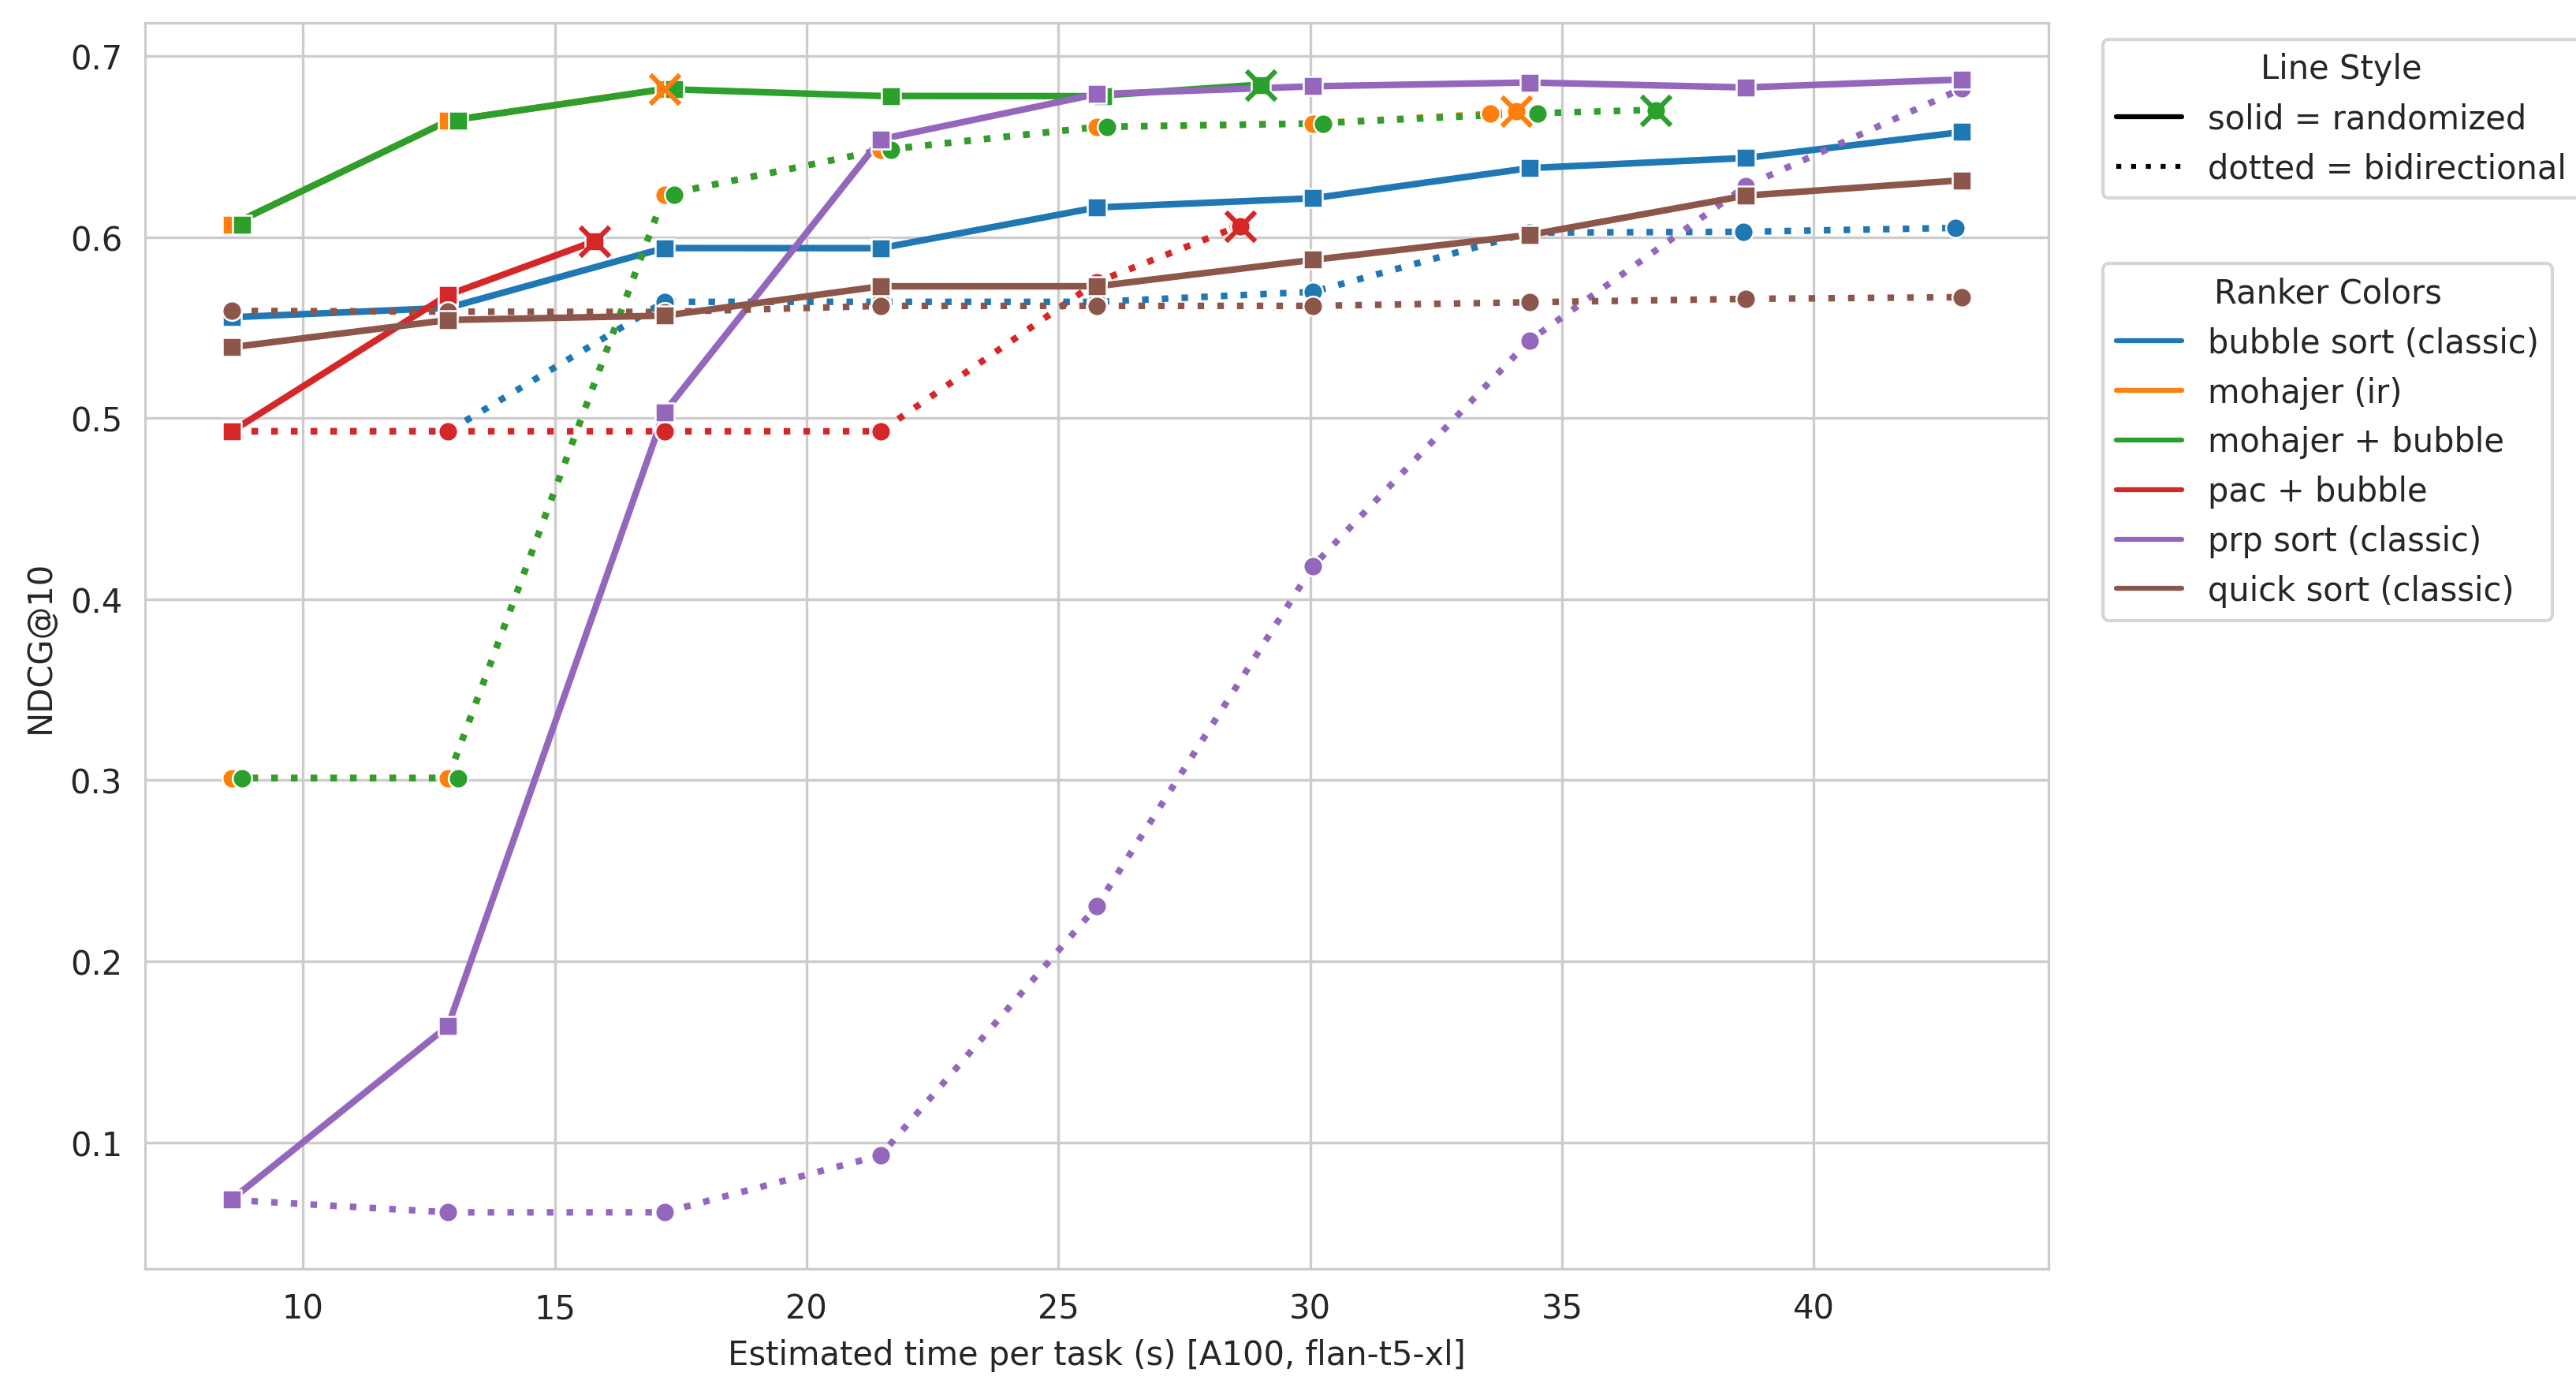
\includegraphics[width=1\linewidth]{reports/figures/limit_comparisons_time/limit_comparisons_time_all_flan_a100_both.png}
    \caption{TREC DL 2019 and DL 2020 (Flan-T5-XL, A100): NDCG@10 vs average time per task. Colors denote rankers; solid lines are randomized and dotted lines are bidirectional. Peak markers (X) are shown for Mohajer/PAC variants.}
    \label{fig:limit_time_all_flan_a100}
\end{figure}
The trend matches the budgeted view: active ranking reaches strong top-$K$ quality earlier (Mohajer fully converges by 23.3s, PAC by 10.1s), while sorting improves more gradually and may overtake only at longer runtimes.


%\section{Conclusion}
%We argue that LLM reranking is better modeled as budgeted learning from noisy pairwise comparisons than as deterministic sorting with an LLM comparator.
%Across IR benchmarks, active ranking methods provide a better NDCG@10--cost/latency trade-off in the call-constrained regime most relevant for top-$K$ context construction, while classical sorting can become competitive only at high budgets.
%Finally, a randomized-direction oracle reduces per-pair prompting cost to a single call and pairs especially well with active schedules, improving quality per call (and per second) without changing the pairwise-PRP interface.




% We first compare active-ranking methods to sorting-based PRP pipelines under the bidirectional oracle (\S\ref{sec:ar-vs-sorting}),
% then study randomized-direction (stochastic) oracles (\S\ref{sec:stochastic-oracle-vs-sorting}).
% Finally, we report anytime effectiveness under fixed inference-call budgets to model query-time constraints (\S\ref{sec:budget_curves}).


%\section{Results and Discussion}



%We take Table~\ref{tab:budget_ndcg10_oracles_flan_xl} as our primary view of effectiveness under strict comparison budgets, reporting average NDCG@10 over TREC DL2019 and DL2020 with Flan-T5-XL. We first interpret the bidirectional-oracle results (\S\ref{sec:ar-vs-sorting}) and then analyze how switching to randomized-direction prompting changes warm-up behavior and the high-budget regime (\S\ref{sec:stochastic-oracle-vs-sorting}). Full budget curves are deferred to the appendix.%
%\footnote{Mohajer+Bubble applies BubbleSort refinement only after the Mohajer stage completes; when the budget is exhausted before that point, Mohajer+Bubble reduces to Mohajer. In Table~\ref{tab:budget_ndcg10_oracles_flan_xl}, this yields identical entries up to $B=350$ in the bidirectional block and up to $B=200$ in the randomized block.}

%\subsection{Active ranking vs.\ classic sorting}
%\label{sec:ar-vs-sorting}

%We interpret the bidirectional-oracle results (top block of Table~\ref{tab:budget_ndcg10_oracles_flan_xl}) from a budgeted perspective, where the goal is to maximize NDCG@10 under a limited number of pairwise comparisons.

%\paragraph{Very low budgets reflect incomplete initialization.}
%At $B\in\{100,150\}$ the active-ranking methods are still in an initialization phase and cannot reliably output a high-quality top-$K$ ordering, producing an apparent ``warm-up'' region.
%In contrast, classic sorting baselines can emit a plausible partial order immediately: QuickSort reaches $\approx 55.9$ NDCG@10 already at $B\in\{100,150\}$, while the Mohajer methods remain much lower (30.12), consistent with not yet meeting the minimum comparison requirements to form a stable candidate set for top-$K$ selection.
%This warm-up ends earlier for the Mohajer family (between $B=150$ and $B=200$, where it jumps to 62.34) than for PAC+Bubble (between $B=250$ and $B=300$, where it first improves above 49.27).

%\paragraph{Low-to-mid budgets: active ranking yields large gains.}
%Once initialized, active ranking dominates the call-constrained regime most relevant for reranking.
%The Mohajer family is best from $B=200$ through $B=450$, improving steadily from 62.34 (at $B=200$) to 67.02 (at $B=450$).%
%\footnote{Within this range, Mohajer and Mohajer+Bubble coincide through $B=350$; beyond that, the refinement variant is slightly higher (e.g., 66.83 vs.\ 66.81 at $B=400$).}
%Relative to the strongest classic sorter at matched budgets, the gains are substantial: at $B=300$, Mohajer achieves 66.09 versus 56.42 for the best classical baseline (BubbleSort), a $+9.67$ NDCG@10 point improvement; at $B=350$, 66.28 versus 56.98 ($+9.30$).
%Even when the best classic baseline strengthens at higher budgets (e.g., HeapSort at $B=450$), the Mohajer family retains a clear advantage (67.02 vs.\ 62.81; $+4.21$).
%PAC+Bubble also surpasses the classic sorting baselines in the mid-budget range (e.g., 60.59 at $B=350$), but it remains consistently below the Mohajer family at matched budgets.

%\paragraph{High budgets: classical sorting catches up.}
%At the largest budget shown ($B=500$), HeapSort continues improving and becomes best (68.21), exceeding the strongest active-ranking variant (67.02).
%This suggests a regime change: once the budget is large enough to sustain continued refinement of a global order, classical sorting can overtake methods optimized for early, top-$K$-focused performance.

%\paragraph{Takeaway.}
%Under the bidirectional oracle, active ranking pays an initialization cost but is decisively better in the low-to-mid budget region ($B\approx 200$--$450$), delivering up to $\sim 10$ NDCG@10 points over classic sorting around $B=300$.
%Classic sorting becomes preferable only at the highest budgets shown, where continued global-order refinement is affordable.

%\subsection{Randomized-direction oracle: effects on active ranking and classic sorting}
%\label{sec:stochastic-oracle-vs-sorting}

%We now switch to randomized-direction prompting (bottom block of Table~\ref{tab:budget_ndcg10_oracles_flan_xl}). Relative to \S\ref{sec:ar-vs-sorting}, the main changes are (i) a much shorter warm-up across methods and (ii) an earlier crossover point where the best classic sorter overtakes active ranking.

%\paragraph{Warm-up is compressed for all methods, and nearly vanishes for Mohajer.}
%Randomized direction moves systems into their effective operating regime with fewer comparisons.
%Most notably, Mohajer is already strong at $B=100$ (60.68), whereas under the bidirectional oracle it is still in warm-up at the same budget (30.12).
%PAC+Bubble also initializes earlier, rising to 56.81 by $B=150$ and 59.78 by $B=200$, compared to being flat through $B\le 250$ under the bidirectional oracle.
%Overall, randomized direction reduces the early-budget penalty associated with methods that require a minimum number of comparisons before producing reliable top-$K$ outputs.

%\paragraph{Active ranking: dominates from the start and converges by 200 comparisons.}
%With randomized direction, active ranking becomes the best option immediately and reaches its plateau extremely quickly.
%Mohajer leads at $B=100$ (60.68) and $B=150$ (66.42), and it effectively converges by $B=200$ (68.18), remaining at 68.18 through $B=500$.
%Moreover, the ``refine-after-converge'' variant attains the strongest active-ranking checkpoint at $B=350$ (Mohajer+Bubble at 68.39), so active ranking remains best from $B=100$ through $B=350$.
%This is also a strict improvement over bidirectional prompting in the call-constrained regime: at $B=200$, Mohajer increases from 62.34 (bidirectional) to 68.18 (randomized), a $+5.84$ gain, while the warm-up region largely disappears.

%\paragraph{Convergence speed: comparable quality with roughly half the budget.}
%A key operational implication is that Mohajer reaches the $\sim$68 NDCG@10 range with only 200 comparisons, while HeapSort requires substantially more budget to reach comparable effectiveness (68.33 at $B=350$ and 68.54 at $B=400$).
%Thus, randomized direction yields a ``win--win'' for active ranking: fewer required comparisons to reach peak quality, and higher quality at matched low budgets.

%\paragraph{High budgets: classic sorting catches up earlier, but the gap is small.}
%Randomized direction also benefits classic sorting enough that the crossover occurs earlier than in \S\ref{sec:ar-vs-sorting}.
%HeapSort overtakes active ranking starting at $B=400$ (68.54 vs.\ 68.18) and remains best through $B=500$ (68.71).
%However, the margin is narrow (e.g., 0.36 at $B=400$), indicating that active ranking stays highly competitive even after classic sorting becomes best at higher budgets.

%\paragraph{Classic sorting improves broadly (especially HeapSort).}
%Among classical pipelines, HeapSort exhibits the most dramatic shift at low budgets: it rises from 6.13 at $B=200$ (bidirectional) to 50.32 at $B=200$ (randomized), and from 41.84 at $B=350$ to 68.33.
%BubbleSort also benefits consistently (e.g., 55.57 at $B=100$ vs.\ 49.27; 65.80 at $B=500$ vs.\ 60.51).
%QuickSort improves primarily in the mid-to-high budget regime (e.g., 63.14 at $B=500$ vs.\ 56.68), even though its very low-budget checkpoints are similar.

%\paragraph{Takeaway.}
%Randomized-direction prompting shortens warm-up across methods and makes active ranking immediately effective: Mohajer converges by $B=200$ and dominates from $B=100$ through $B=350$, improving over bidirectional prompting at the same budgets.
%Classic sorting---especially HeapSort---also improves substantially and becomes best at higher budgets ($B\ge 400$), shifting the crossover earlier than under the bidirectional oracle.


% \subsection{Active ranking with Stochastic Oracles vs. classic sorting}

% \paragraph{Fixed-budget interpretation.}
% Several comparisons in Section~\ref{sec:results} are most naturally interpreted under a \emph{fixed inference-call budget}.
% Bidirectional prompting spends two calls per match, so it executes fewer distinct matches than randomized-direction at the same budget.
% Accordingly, performance reflects a trade-off between (i) per-match reliability (favoring bidirectional) and (ii) coverage over distinct pairs (favoring randomized-direction).
%  %% Agregaria como una sub sub section el grafico de limit comparisons, no como titulo. Main es Active con Sampling . 

% \paragraph{Discussion.}
% At a fixed call budget, sampling often improves NDCG@10 for methods that benefit from more distinct pairwise evidence (notably PRP sort on TREC-COVID), even though each individual comparison is noisier.
% However, the effect is dataset-dependent: on SciFact, bubble sort with bidirectional prompting remains stronger than sampling across much of the budget range in your table.
% Overall, the budgeted results suggest that \emph{call-efficiency} is governed by two interacting factors: (i) per-match reliability (favoring bidirectional) and (ii) the number of distinct matches (favoring sampling).

\section{Conclusion}
We argue that PRP LLM reranking is better modeled as budgeted learning from noisy pairwise comparisons than as deterministic sorting.
Empirically, active rankers deliver stronger NDCG@10 in the call-constrained regime, while sorting becomes preferable only at large budgets where global-order refinement is affordable.
Moreover, randomized-direction prompting (one call per pair) pairs particularly well with active schedules by enabling more distinct comparisons under a fixed budget.
Additional end-to-end and budgeted results are reported in the appendix.


%\section{Conclusion}
%We frame LLM reranking as ranking from noisy pairwise comparisons and evaluate two practical efficiency levers.
%First, active ranking procedures can reduce LLM calls by an order of magnitude relative to classic bidirectional sorting pipelines in our runs, at the cost of a moderate reduction in average NDCG@10.
%Second, under a fixed LLM-call budget, single-call (sampling/randomized-direction) comparisons can be more effective than bidirectional prompting because they enable more distinct matches, although the benefit is dataset- and algorithm-dependent.
%Future work should replicate these trends with live LLM APIs (to capture latency, batching, and nonstationarity effects), and characterize when doubling match count outweighs the loss in per-match reliability.

\section*{Limitations}

Our study focuses on reranking settings where a reliable pairwise LLM comparator can be elicited with constrained outputs. Results may vary with prompt design, model family, and decoding settings. Our cost metric counts LLM calls (and optionally tokens) but does not capture all system-level overheads (e.g., batching constraints, caching, network latency).

The observed NDCG@10 improvements from randomized-direction oracles on active rankers, while consistent across our experiments, require further theoretical investigation. The hypothesis that independent single-direction samples benefit adaptive algorithms more than correlated bidirectional samples is plausible but not rigorously proven. Alternative explanations warrant dedicated analysis.

Our PAC Optimized method introduces a candidate pool multiplier hyperparameter $m$ (default $m=3$), which controls the trade-off between comparison cost and coverage of the prior ranking. We did not perform a systematic ablation over $m$ due to computational constraints, and the optimal value likely depends on prior quality and dataset characteristics. While $m=3$ yields strong empirical results in our experiments, future work should investigate data-driven or adaptive selection strategies for this parameter.

Finally, active ranking theory often assumes conditional independence of oracle outputs; real LLM APIs can violate this through hidden state, caching, or nonstationarity.


\section*{Acknowledgments}
% TODO
We thank [\;] for discussions and feedback.

\clearpage
\FloatBarrier
\bibliographystyle{acl_natbib}
\bibliography{custom}


% ====== APPENDIX (drop-in) ======

\clearpage
\onecolumn        % flushes (internally) BEFORE we start appendix numbering
\appendix

\section{Supplementary Tables}
\label{sec:appendix}
\FloatBarrier

% Anchor the section heading before any appendix floats:
\FloatBarrier

\noindent This appendix provides supplementary results and ablations referenced in the main text.
\vspace{0.5em}

\begingroup

% --- Float tuning (lets LaTeX place multiple tables per page) ---
\setcounter{topnumber}{5}
\setcounter{bottomnumber}{5}
\setcounter{totalnumber}{10}
\renewcommand{\topfraction}{0.95}
\renewcommand{\bottomfraction}{0.95}
\renewcommand{\textfraction}{0.05}
\renewcommand{\floatpagefraction}{0.95}

% --- Local spacing/style for appendix tables ---
\setlength{\textfloatsep}{10pt plus 2pt minus 2pt}
\setlength{\floatsep}{8pt plus 2pt minus 2pt}
\setlength{\intextsep}{8pt plus 2pt minus 2pt}
\renewcommand{\arraystretch}{1.08}
\setlength{\tabcolsep}{3.5pt}

\captionsetup[table]{
  font=small,
  labelfont=bf,
  skip=3pt,
  justification=raggedright,
  singlelinecheck=false
}
\captionsetup[subtable]{
  font=small,
  justification=centering,
  singlelinecheck=false
}

% Appendix-style numbering (Table A.1, A.2, ...)
\setcounter{table}{0}
\renewcommand{\thetable}{A.\arabic{table}}

% Optional safety: avoid redefinition errors if already defined earlier.
\providecommand{\best}[1]{\textbf{#1}}
\providecommand{\second}[1]{\underline{#1}}
\providecommand{\conv}[1]{#1\textsuperscript{\textdagger}}
\providecommand{\postconv}[1]{\textcolor{black!55}{#1}}

% ------------------------------------------------------------
% (A1) Budgeted NDCG@10 over DL2019 and DL2020 (single table, subtables)
% ------------------------------------------------------------
\begin{table}[H]
\centering

\begin{subtable}{\textwidth}
\centering
\caption{TREC DL2019}
\label{tab:budget_ndcg10_oracles_flan_xl_dl2019}
\begin{adjustbox}{max width=\textwidth}
\scriptsize
\begin{tabular}{c l rrrrrrrrr}
\toprule
& & \multicolumn{9}{c}{Number of comparisons (budget)} \\
\cmidrule(lr){3-11}
Oracle & Ranker & 100 & 150 & 200 & 250 & 300 & 350 & 400 & 450 & 500 \\
\midrule
\multirow{6}{*}{\rotatebox[origin=c]{90}{Bidirectional}} & BubbleSort & \underline{50.58} & \underline{50.58} & 57.13 & 57.13 & 57.13 & 57.78 & 60.64 & 60.69 & 60.95 \\
& HeapSort & 9.14 & 8.49 & 8.61 & 11.91 & 23.97 & 41.68 & 54.14 & 63.58 & \textbf{68.92} \\
& QuickSort & \textbf{58.08} & \textbf{58.08} & \underline{58.30} & \underline{58.57} & 58.57 & 58.57 & 58.85 & 59.08 & 59.27 \\
& PAC + Bubble & \underline{50.58} & \underline{50.58} & 50.58 & 50.58 & \underline{60.00} & \underline{62.59} & \underline{62.60} & 62.60 & 62.60 \\
& Mohajer + Bubble & 32.76 & 32.76 & \textbf{62.44} & \textbf{65.35} & \textbf{66.34} & \textbf{66.23} & \textbf{66.64} & \textbf{66.59} & \underline{66.59} \\
& Mohajer & 32.76 & 32.76 & \textbf{62.44} & \textbf{65.35} & \textbf{66.34} & \textbf{66.23} & \textbf{66.64} & \underline{66.58} & 66.58 \\
\midrule
\multirow{6}{*}{\rotatebox[origin=c]{90}{Randomized}} & BubbleSort & 55.92 & 56.88 & 59.77 & 60.33 & 61.98 & 62.52 & 64.27 & 64.37 & 65.73 \\
& HeapSort & 9.11 & 16.89 & 49.27 & 65.93 & 68.49 & \underline{69.03} & \textbf{69.82} & \underline{68.76} & \underline{68.84} \\
& QuickSort & \underline{56.33} & 57.57 & 56.98 & 59.89 & 58.42 & 61.44 & 63.00 & 64.83 & 64.37 \\
& PAC + Bubble & 50.58 & \underline{58.35} & \underline{61.05} & 61.05 & 61.05 & 61.05 & 61.05 & 61.05 & 61.05 \\
& Mohajer + Bubble & \textbf{61.41} & \textbf{67.79} & \textbf{68.70} & \underline{67.99} & \underline{68.53} & \textbf{69.17} & \underline{69.47} & \textbf{69.47} & \textbf{69.47} \\
& Mohajer & \textbf{61.41} & \textbf{67.79} & \textbf{68.70} & \textbf{68.73} & \textbf{68.73} & 68.73 & 68.73 & 68.73 & 68.73 \\
\bottomrule
\end{tabular}
\end{adjustbox}
\end{subtable}

\vspace{0.35em}

\begin{subtable}{\textwidth}
\centering
\caption{TREC DL2020}
\label{tab:budget_ndcg10_oracles_flan_xl_dl2020}
\begin{adjustbox}{max width=\textwidth}
\scriptsize
\begin{tabular}{c l rrrrrrrrr}
\toprule
& & \multicolumn{9}{c}{Number of comparisons (budget)} \\
\cmidrule(lr){3-11}
Oracle & Ranker & 100 & 150 & 200 & 250 & 300 & 350 & 400 & 450 & 500 \\
\midrule
\multirow{6}{*}{\rotatebox[origin=c]{90}{Bidirectional}} & BubbleSort & \underline{47.96} & \underline{47.96} & \underline{55.72} & \underline{55.72} & \underline{55.72} & 56.18 & 59.86 & 59.90 & 60.07 \\
& HeapSort & 4.48 & 3.77 & 3.65 & 6.65 & 22.12 & 42.00 & 54.44 & 62.05 & \textbf{67.50} \\
& QuickSort & \textbf{53.77} & \textbf{53.69} & 53.44 & 53.83 & 53.83 & 53.83 & 53.95 & 54.10 & 54.10 \\
& PAC + Bubble & \underline{47.96} & \underline{47.96} & 47.96 & 47.96 & 55.04 & \underline{58.59} & \underline{58.62} & 58.62 & 58.62 \\
& Mohajer + Bubble & 27.48 & 27.48 & \textbf{62.24} & \textbf{64.25} & \textbf{65.83} & \textbf{66.32} & \textbf{67.02} & \textbf{67.45} & \underline{67.45} \\
& Mohajer & 27.48 & 27.48 & \textbf{62.24} & \textbf{64.25} & \textbf{65.83} & \textbf{66.32} & \underline{66.98} & \underline{67.35} & 67.35 \\
\midrule
\multirow{6}{*}{\rotatebox[origin=c]{90}{Randomized}} & BubbleSort & \underline{55.23} & \underline{55.31} & \underline{59.03} & 58.45 & 61.30 & 61.78 & 63.35 & 64.37 & 65.88 \\
& HeapSort & 4.59 & 15.96 & 51.38 & 64.88 & \underline{67.31} & \textbf{67.64} & \underline{67.27} & \underline{67.78} & \textbf{68.58} \\
& QuickSort & 51.51 & 53.28 & 54.34 & 54.67 & 56.15 & 56.05 & 57.25 & 59.76 & 61.91 \\
& PAC + Bubble & 47.96 & 55.27 & 58.51 & 58.51 & 58.51 & 58.51 & 58.51 & 58.51 & 58.51 \\
& Mohajer + Bubble & \textbf{59.95} & \textbf{65.06} & \textbf{67.66} & \underline{67.61} & 67.05 & \underline{67.60} & 66.30 & 66.30 & 66.30 \\
& Mohajer & \textbf{59.95} & \textbf{65.06} & \textbf{67.66} & \textbf{67.62} & \textbf{67.62} & \textbf{67.62} & \textbf{67.62} & \textbf{67.62} & \underline{67.62} \\
\bottomrule
\end{tabular}
\end{adjustbox}
\end{subtable}

\caption{
Budgeted NDCG@10 (\%) on TREC DL2019 and DL2020 using Flan-T5-XL under bidirectional vs.\ randomized-direction prompting.
Budgets denote the number of pairwise comparisons. Within each oracle block, bold/underline indicate best/second-best per budget column among the listed rankers.
}
\label{tab:budget_ndcg10_oracles_flan_xl_by_dataset}
\end{table}
% ------------------------------------------------------------
% (A2) Top-k sweep under randomized-direction prompting (Flan-T5-XL)
% ------------------------------------------------------------
\begin{table}[H]
\centering
\small
\begin{adjustbox}{max width=\textwidth}
\begin{tabular}{c l rrrrrrrrr}
\toprule
& & \multicolumn{9}{c}{Number of comparisons (budget)} \\
\cmidrule(lr){3-11}
$k$ & Ranker & 100 & 150 & 200 & 250 & 300 & 350 & 400 & 450 & 500 \\
\midrule
\multirow{2}{*}{10} & BubbleSort
& 55.57 & 56.10 & 59.40 & 59.39 & 61.64 & 62.15 & 63.81 & 64.37 & 65.80 \\
& Mohajer
& \best{60.68} & \best{66.42} & \conv{\best{68.18}} & \postconv{\best{68.18}} & \postconv{\best{68.18}} & \postconv{\best{68.18}} & \postconv{\best{68.18}} & \postconv{\best{68.18}} & \postconv{\best{68.18}} \\
\midrule
\multirow{2}{*}{20} & BubbleSort
& \best{52.73} & 53.07 & 55.76 & 55.62 & 57.36 & 57.60 & 59.18 & 59.31 & 60.49 \\
& Mohajer
& 51.51 & \best{58.30} & \best{61.82} & \conv{\best{62.98}} & \postconv{\best{62.98}} & \postconv{\best{62.98}} & \postconv{\best{62.98}} & \postconv{\best{62.98}} & \postconv{\best{62.98}} \\
\midrule
\multirow{2}{*}{30} & BubbleSort
& \best{51.62} & 52.02 & 54.06 & 53.88 & 55.49 & 55.61 & 57.07 & 57.19 & 58.02 \\
& Mohajer
& 48.61 & \best{54.04} & \best{56.69} & \conv{\best{58.22}} & \postconv{\best{58.22}} & \postconv{\best{58.22}} & \postconv{\best{58.22}} & \postconv{\best{58.22}} & \postconv{\best{58.22}} \\
\midrule
\multirow{2}{*}{40} & BubbleSort
& \best{51.47} & 51.78 & 53.77 & 53.58 & 55.17 & 55.44 & \best{56.38} & \best{56.86} & \best{57.19} \\
& Mohajer
& 48.06 & \best{52.94} & \best{54.49} & \conv{\best{56.03}} & \postconv{\best{56.03}} & \postconv{\best{56.03}} & \postconv{56.03} & \postconv{56.03} & \postconv{56.03} \\
\midrule
\multirow{2}{*}{50} & BubbleSort
& \best{51.46} & 52.38 & 53.59 & 53.83 & 54.71 & \best{55.31} & \best{55.80} & \best{56.17} & \best{56.49} \\
& Mohajer
& 48.12 & \best{52.72} & \best{53.96} & \conv{\best{55.03}} & \postconv{\best{55.03}} & \postconv{55.03} & \postconv{55.03} & \postconv{55.03} & \postconv{55.03} \\
\bottomrule
\end{tabular}
\end{adjustbox}
\caption{
Top-$k$ sweep with randomized-direction prompting (Flan-T5-XL). Values are average NDCG@$k$ (\%) over TREC DL2019 and DL2020.
Budgets denote the number of pairwise comparisons. For each $(k,\text{budget})$, bold marks the better of BubbleSort vs.\ Mohajer.
\textsuperscript{\textdagger} indicates the first budget where the method is treated as converged; subsequent budgets are de-emphasized.
}
\label{tab:k_budget_sweep_randomized}
\par\vspace{2pt}\footnotesize\noindent\textit{Note.} Mohajer dominates BubbleSort when $k$ and the budget are low. As $k$ increases, the crossover point where BubbleSort overtakes Mohajer arrives sooner in terms of number of comparisons.
\end{table}
% ------------------------------------------------------------
% (A3) PRP-Graph comparison
% ------------------------------------------------------------
\begin{table}[H]
\centering
\small
\begin{adjustbox}{max width=\textwidth}
\begin{tabular}{@{}llcccc@{}}
\toprule
\multirow{2}{*}{LLM} & \multirow{2}{*}{Method}
& \multicolumn{2}{c}{DL2019}
& \multicolumn{2}{c}{DL2020} \\
\cmidrule(lr){3-4}\cmidrule(lr){5-6}
& & NDCG@10 (\%) & \#Inf. & NDCG@10 (\%) & \#Inf. \\
\midrule
NA & BM25 & 50.6 & -- & 48.0 & -- \\
\midrule
\multirow{3}{*}{Flan-T5-L}
& PRP-Graph-10     & \best{65.8}    & 492.7  & \best{61.8}    & 492.5  \\
& Mohajer + Bu. & \second{61.75} & 354.60 & \second{58.8}  & 354.245 \\
& PAC + Bu.     & 59.9           & 183.34 & 57.29          & 183.99 \\
\midrule
\multirow{3}{*}{Flan-T5-XL}
& PRP-Graph-10     & \second{67.6}  & 492.6  & \second{66.1}  & 492.5 \\
& Mohajer + Bu. & \best{69.47}   & 338.11 & \best{66.3}    & 338.74 \\
& PAC + Bu.     & 61.05          & 184.16 & 58.51          & 183.72 \\
\midrule
\multirow{3}{*}{Flan-T5-XXL}
& PRP-Graph-10     & \second{66.6}  & 492.6  & \second{66.1}  & 492.6 \\
& Mohajer + Bu. & \best{68.54}   & 341.81 & \best{68.96}   & 344.17 \\
& PAC + Bu.     & 60.92          & 183.46 & 60.71          & 183.59 \\
\bottomrule
\end{tabular}
\end{adjustbox}
\caption{
Comparison to PRP-Graph on TREC DL2019/2020. NDCG@10 is reported in percent.
“\#Inf.” is the average number of inferred pairwise comparisons used by the method (lower is fewer comparisons).
Bold/underline indicate best/second-best NDCG@10 within each (DL year, LLM) block.
}
\label{tab:trec_prpgraph_comp}
\par\vspace{2pt}\footnotesize\noindent\textit{Note.} Our results show that with larger Flan models, Mohajer + Bubble has increasingly better results than PRP-Graph with less comparisons. PAC + Bubble falls behind in performance but has significantly less comparisons. 
\end{table}
% ------------------------------------------------------------
% (A4) End-to-end table (single-column; keep as table, not table*)
% ------------------------------------------------------------
\begin{table}[H]
\centering
\footnotesize
\setlength{\tabcolsep}{3pt}
\renewcommand{\arraystretch}{1.12}
\begin{adjustbox}{max width=\textwidth}
\begin{tabular}{llcccccccccc}
\toprule
\multicolumn{2}{c}{\textbf{Method}} &
\multicolumn{8}{c}{\textbf{Dataset (NDCG@10 \%)}} &
\textbf{Avg. NDCG@10} & \textbf{Avg. Calls/Task} \\
\cmidrule(lr){1-2}\cmidrule(lr){3-10}\cmidrule(lr){11-12}
\textbf{Reranker} & \textbf{Oracle} &
\textbf{Covid} & \textbf{Robust04} & \textbf{Touche} & \textbf{SciFact} &
\textbf{DBPedia} & \textbf{DL19} & \textbf{DL20} & \textbf{FiQA} & & \\
\midrule
% ---- (keep your existing body unchanged) ----
\multirow{2}{*}{BubbleSort} & Bidirectional
& 70.9 & 44.2 & \textbf{44.7} & \textbf{69.2} & 41.7 & 63.4 & 58.6 & 29.4 & 52.8 & \textbf{766} \\
& Randomized
& \textbf{74.9} & \textbf{45.8} & 41.2 & 67.2 & \textbf{43.6} & \textbf{67.6} & \textbf{63.9} & \textbf{32.3} & \textbf{54.6} & 4084 \\
\midrule
\multirow{2}{*}{HeapSort} & Bidirectional
& 76.0 & \textbf{40.4} & \textbf{33.2} & \textbf{67.5} & \textbf{41.4} & \textbf{65.0} & \textbf{62.6} & \textbf{31.3} & \textbf{52.7} & 1230 \\
& Randomized
& \textbf{76.9} & 38.4 & 27.7 & 63.3 & 39.8 & 62.6 & 58.5 & 27.7 & 49.0 & \textbf{860} \\
\midrule
\multirow{2}{*}{QuickSort} & Bidirectional
& \textbf{76.2} & \textbf{41.0} & \textbf{27.4} & \textbf{60.1} & \textbf{41.1} & \textbf{64.5} & \textbf{58.5} & \textbf{26.8} & \textbf{49.5} & 1954 \\
& Randomized
& 75.8 & 35.4 & 25.1 & 58.7 & 39.1 & 61.8 & 58.1 & 24.6 & 47.3 & \textbf{556} \\
\midrule
\multirow{2}{*}{Mohajer} & Bidirectional
& \textbf{76.5} & \textbf{37.5} & \textbf{26.4} & 53.8 & \textbf{39.7} & \textbf{62.6} & 56.1 & \textbf{25.9} & \textbf{47.3} & 399 \\
& Randomized
& 76.2 & 36.2 & 24.4 & \textbf{57.5} & 39.1 & 60.6 & \textbf{57.2} & 24.9 & 47.0 & \textbf{232} \\
\midrule
\multirow{2}{*}{Mohajer+Bubble} & Bidirectional
& 76.5 & 37.5 & \textbf{26.4} & 53.9 & 39.7 & \textbf{62.6} & 56.1 & 25.9 & 47.3 & 423 \\
& Randomized
& \textbf{76.9} & \textbf{37.8} & 25.7 & \textbf{58.8} & \textbf{40.0} & 61.8 & \textbf{58.8} & \textbf{26.2} & \textbf{48.2} & \textbf{354} \\
\midrule
\multirow{2}{*}{Pac+Bubble} & Bidirectional
& 69.3 & \textbf{44.0} & \textbf{41.4} & \textbf{68.5} & \textbf{39.2} & \textbf{61.7} & 57.2 & \textbf{29.2} & \textbf{51.3} & 323 \\
& Randomized
& \textbf{70.2} & 41.0 & 38.2 & 67.0 & 38.1 & 60.0 & \textbf{57.3} & 27.2 & 49.9 & \textbf{184} \\
\bottomrule
\end{tabular}
\end{adjustbox}
\caption{
End-to-end NDCG@10 (\%) and average pairwise-comparison calls per task. For each reranker and column, \textbf{bold} indicates the better oracle variant (higher NDCG; lower calls).
If the two oracle variants tie after rounding, both are bolded. % !!Modelo?
}
\label{tab:reranker_oracle_compare}
\par\vspace{2pt}\footnotesize\noindent\textit{Note.} Active-learning rankers are more robust to noisy comparisons and profit most from randomized-direction sampling. Bubblesort requires many more comparisons as cycles emerge, but said cycles allow the latent transitive ordering to surface more than with a deterministic oracle, yielding higher NDCG@10.

\end{table}

% ------------------------------------------------------------
% Bidirectional flip-rate sanity check (order effects)
% Paste this in the Appendix where you want the tables to appear.
% ------------------------------------------------------------
\begin{table*}[H]
\centering
\small
\renewcommand{\arraystretch}{1.15}
\setlength{\tabcolsep}{6pt}

\begin{minipage}[t]{0.48\textwidth}
\centering
\textbf{Stratified by dataset}\\[2pt]
\begin{tabular}{lrrr}
\hline
Dataset & Flip-rate & \#Pairs & \#Flips \\
\hline
All   & 20.62\% & 1,202,850 & 248,021 \\
DL19  & 21.40\% &   212,850 &  45,542 \\
DL20  & 20.45\% &   990,000 & 202,479 \\
\hline
\end{tabular}
\end{minipage}\hfill
\begin{minipage}[t]{0.48\textwidth}
\centering
\textbf{Stratified by BM25 rank distance $|r(i)-r(j)|$}\\[2pt]
\begin{tabular}{lrrr}
\hline
$|r(i)-r(j)|$ & Flip-rate & \#Pairs & \#Flips \\
\hline
1--5    & 22.56\% &  92,639 &  20,903 \\
6--10   & 20.73\% &  86,645 &  17,965 \\
11--20  & 20.85\% & 160,762 &  33,524 \\
$>20$   & 20.36\% & 862,804 & 175,629 \\
\hline
\end{tabular}
\end{minipage}

\caption{Bidirectional flip-rate sanity check (order effects). For each candidate pair $\{d_i,d_j\}$, we query the judge twice—once as $(d_i,d_j)$ and once as $(d_j,d_i)$—and report the fraction of pairs whose winner flips. Results are shown overall and stratified by dataset and BM25 rank distance.}
\label{tab:flip_rate_order_effects}
\end{table*}

\begin{table*}[H]
\centering
\begin{adjustbox}{max width=\textwidth}
\scriptsize
\begin{tabular}{c l rrrrrrrrr}
\toprule
& & \multicolumn{9}{c}{Number of comparisons (budget)} \\
\cmidrule(lr){3-11}
Oracle & Ranker & 100 & 150 & 200 & 250 & 300 & 350 & 400 & 450 & 500 \\
\midrule

\multirow{6}{*}{\rotatebox[origin=c]{90}{Bidirectional}}
& BubbleSort        & \underline{50.58} & \underline{50.58} & 57.04 & 57.04 & 57.18 & 58.73 & 60.98 & 61.30 & 61.90 \\
& HeapSort          & 8.64 & 8.16 & 7.99 & 10.48 & 25.65 & 42.42 & 55.85 & 64.24 & \underline{69.14} \\
& QuickSort         & \textbf{58.28} & \textbf{58.11} & 58.04 & 58.63 & 58.71 & 58.71 & 58.71 & 59.09 & 59.67 \\
& PAC + Bubble      & \underline{50.58} & \underline{50.58} & 50.58 & 50.58 & \underline{60.74} & \conv{\underline{64.25}} & \postconv{64.25} & \postconv{64.25} & \postconv{64.25} \\
& Mohajer + Bubble  & 32.76 & 32.76 & \textbf{62.97} & \textbf{66.69} & \textbf{68.60} & \textbf{69.39} & \textbf{70.08} & \conv{\textbf{70.49}} & \postconv{\textbf{70.49}} \\
& Mohajer           & 32.76 & 32.76 & \textbf{62.97} & \textbf{66.69} & \textbf{68.60} & \textbf{69.39} & \textbf{70.08} & \conv{\underline{70.43}} & \postconv{\underline{70.43}} \\

\midrule

\multirow{6}{*}{\rotatebox[origin=c]{90}{Randomized}}
& BubbleSort        & \underline{57.49} & 57.79 & 61.11 & 61.45 & 64.32 & 64.24 & 66.44 & 66.27 & 67.12 \\
& HeapSort          & 8.20 & 16.13 & 53.18 & \underline{68.15} & \textbf{71.52} & \underline{69.61} & \textbf{70.73} & \textbf{71.14} & \underline{70.70} \\
& QuickSort         & 54.94 & 56.56 & 58.25 & 57.03 & 59.96 & 60.92 & 62.13 & 61.92 & 64.81 \\
& PAC + Bubble      & 50.58 & \underline{57.00} & \conv{\underline{63.02}} & \postconv{63.02} & \postconv{63.02} & \postconv{63.02} & \postconv{63.02} & \postconv{63.02} & \postconv{63.02} \\
& Mohajer + Bubble  & \textbf{63.37} & \textbf{66.49} & \textbf{69.37} & \textbf{68.82} & \underline{70.33} & \textbf{70.44} & \conv{\underline{70.26}} & \postconv{\underline{70.26}} & \postconv{\underline{70.26}} \\
& Mohajer           & \textbf{63.37} & \textbf{66.49} & \underline{69.37} & \conv{\underline{70.98}} & \postconv{\textbf{70.98}} & \postconv{\textbf{70.98}} & \postconv{\textbf{70.98}} & \postconv{\textbf{70.98}} & \postconv{\textbf{70.98}} \\

\bottomrule
\end{tabular}%
\end{adjustbox}
\caption{Average NDCG@10 (\%) on TREC DL 2019 with Qwen3-4B-Instruct across comparison budgets. Bold = best per column; underline = second-best per column (within each oracle block). \textsuperscript{\textdagger} indicates the smallest budget at which a method completes; results at larger budgets are visually de-emphasized.}
\label{tab:budget_ndcg10_oracles_qwen3_4b_dl2019}
\par\vspace{2pt}\footnotesize\noindent\textit{Note.} Though not always the best in performance, active ranking algorithms reach competitive NDCG@10 to the classic algorithms, with drastic improvements in terms of average calls per task.


\end{table*}


% ------------------------------------------------------------
% (AX) Qwen3-4B-Instruct end-to-end table (compact; DL19/DL20 only)
%  - "Sampling" -> "Randomized"
%  - "PRP" corresponds to HeapSort (shown as HeapSort below)
%  - Only our methods include both oracles (PAC+Bubble, Mohajer variants)
% ------------------------------------------------------------
\begin{table*}[H]
\centering
\scriptsize
\setlength{\tabcolsep}{2.0pt}
\renewcommand{\arraystretch}{1.00}
\resizebox{0.90\textwidth}{!}{%
\begin{tabular}{llrrrr}
\toprule
\multicolumn{2}{c}{\textbf{Method}} &
\multicolumn{2}{c}{\textbf{Dataset (NDCG@10 \%)}} &
\textbf{Avg. NDCG@10} & \textbf{Avg. Calls/Task} \\
\cmidrule(lr){1-2}\cmidrule(lr){3-4}\cmidrule(lr){5-6}
& \textbf{Ranker (Oracle)} & \textbf{DL19} & \textbf{DL20} & & \\
\midrule
& \textbf{BM25} & 50.60 & 48.00 & 49.30 & -- \\
\midrule

\multirow{9}{*}{\rotatebox{90}{\textbf{Qwen3-4B-Instruct}}}
& BubbleSort (Bidirectional) & 67.44 & \textbf{70.45} & 68.95 & 1062.69 \\
& HeapSort (Bidirectional)   & 70.26 & \underline{69.46} & \textbf{69.86} & 1383.02 \\
& QuickSort (Bidirectional)  & \underline{70.70} & 68.83 & \underline{69.77} & 1567.02 \\
% --- gray/dampened separator between baselines and ours
\arrayrulecolor{black!35}
\cmidrule(lr){2-6}
\arrayrulecolor{black}
& PAC + Bubble (Bidirectional) & 64.25 & 67.09 & 65.67 & 332.55 \\
& PAC + Bubble (Randomized)    & 63.02 & 66.05 & 64.54 & \textbf{183.42} \\
& Mohajer + Bubble (Bidirectional) & 70.49 & 66.92 & 68.70 & 425.67 \\
& Mohajer + Bubble (Randomized)    & 70.26 & 67.58 & 68.92 & 346.54 \\
& Mohajer (Bidirectional)          & 70.43 & 66.92 & 68.67 & 398.26 \\
& Mohajer (Randomized)             & \textbf{70.98} & 65.43 & 68.20 & \underline{232.01} \\
\bottomrule
\end{tabular}%
}
\caption{
TREC DL2019/2020 end-to-end NDCG@10 (\%) and average pairwise-comparison calls per task using \textbf{Qwen3-4B-Instruct}.
Baselines are reported with a bidirectional oracle; our methods (PAC+Bubble and Mohajer variants) include both bidirectional and randomized comparisons.
Within the Qwen block, best is bold and second-best is underlined per column (higher NDCG; lower calls).
}
\label{tab:qwen3_4b_end2end}

\par\vspace{2pt}\footnotesize\noindent\textit{Note.} Though not always the best in performance, active ranking algorithms reach competitive NDCG@10 to the classic algorithms, with drastic improvements in terms of average calls per task.

\end{table*}


\begin{figure}[H]
    \centering
    \begin{subfigure}[t]{0.48\linewidth}
        \centering
        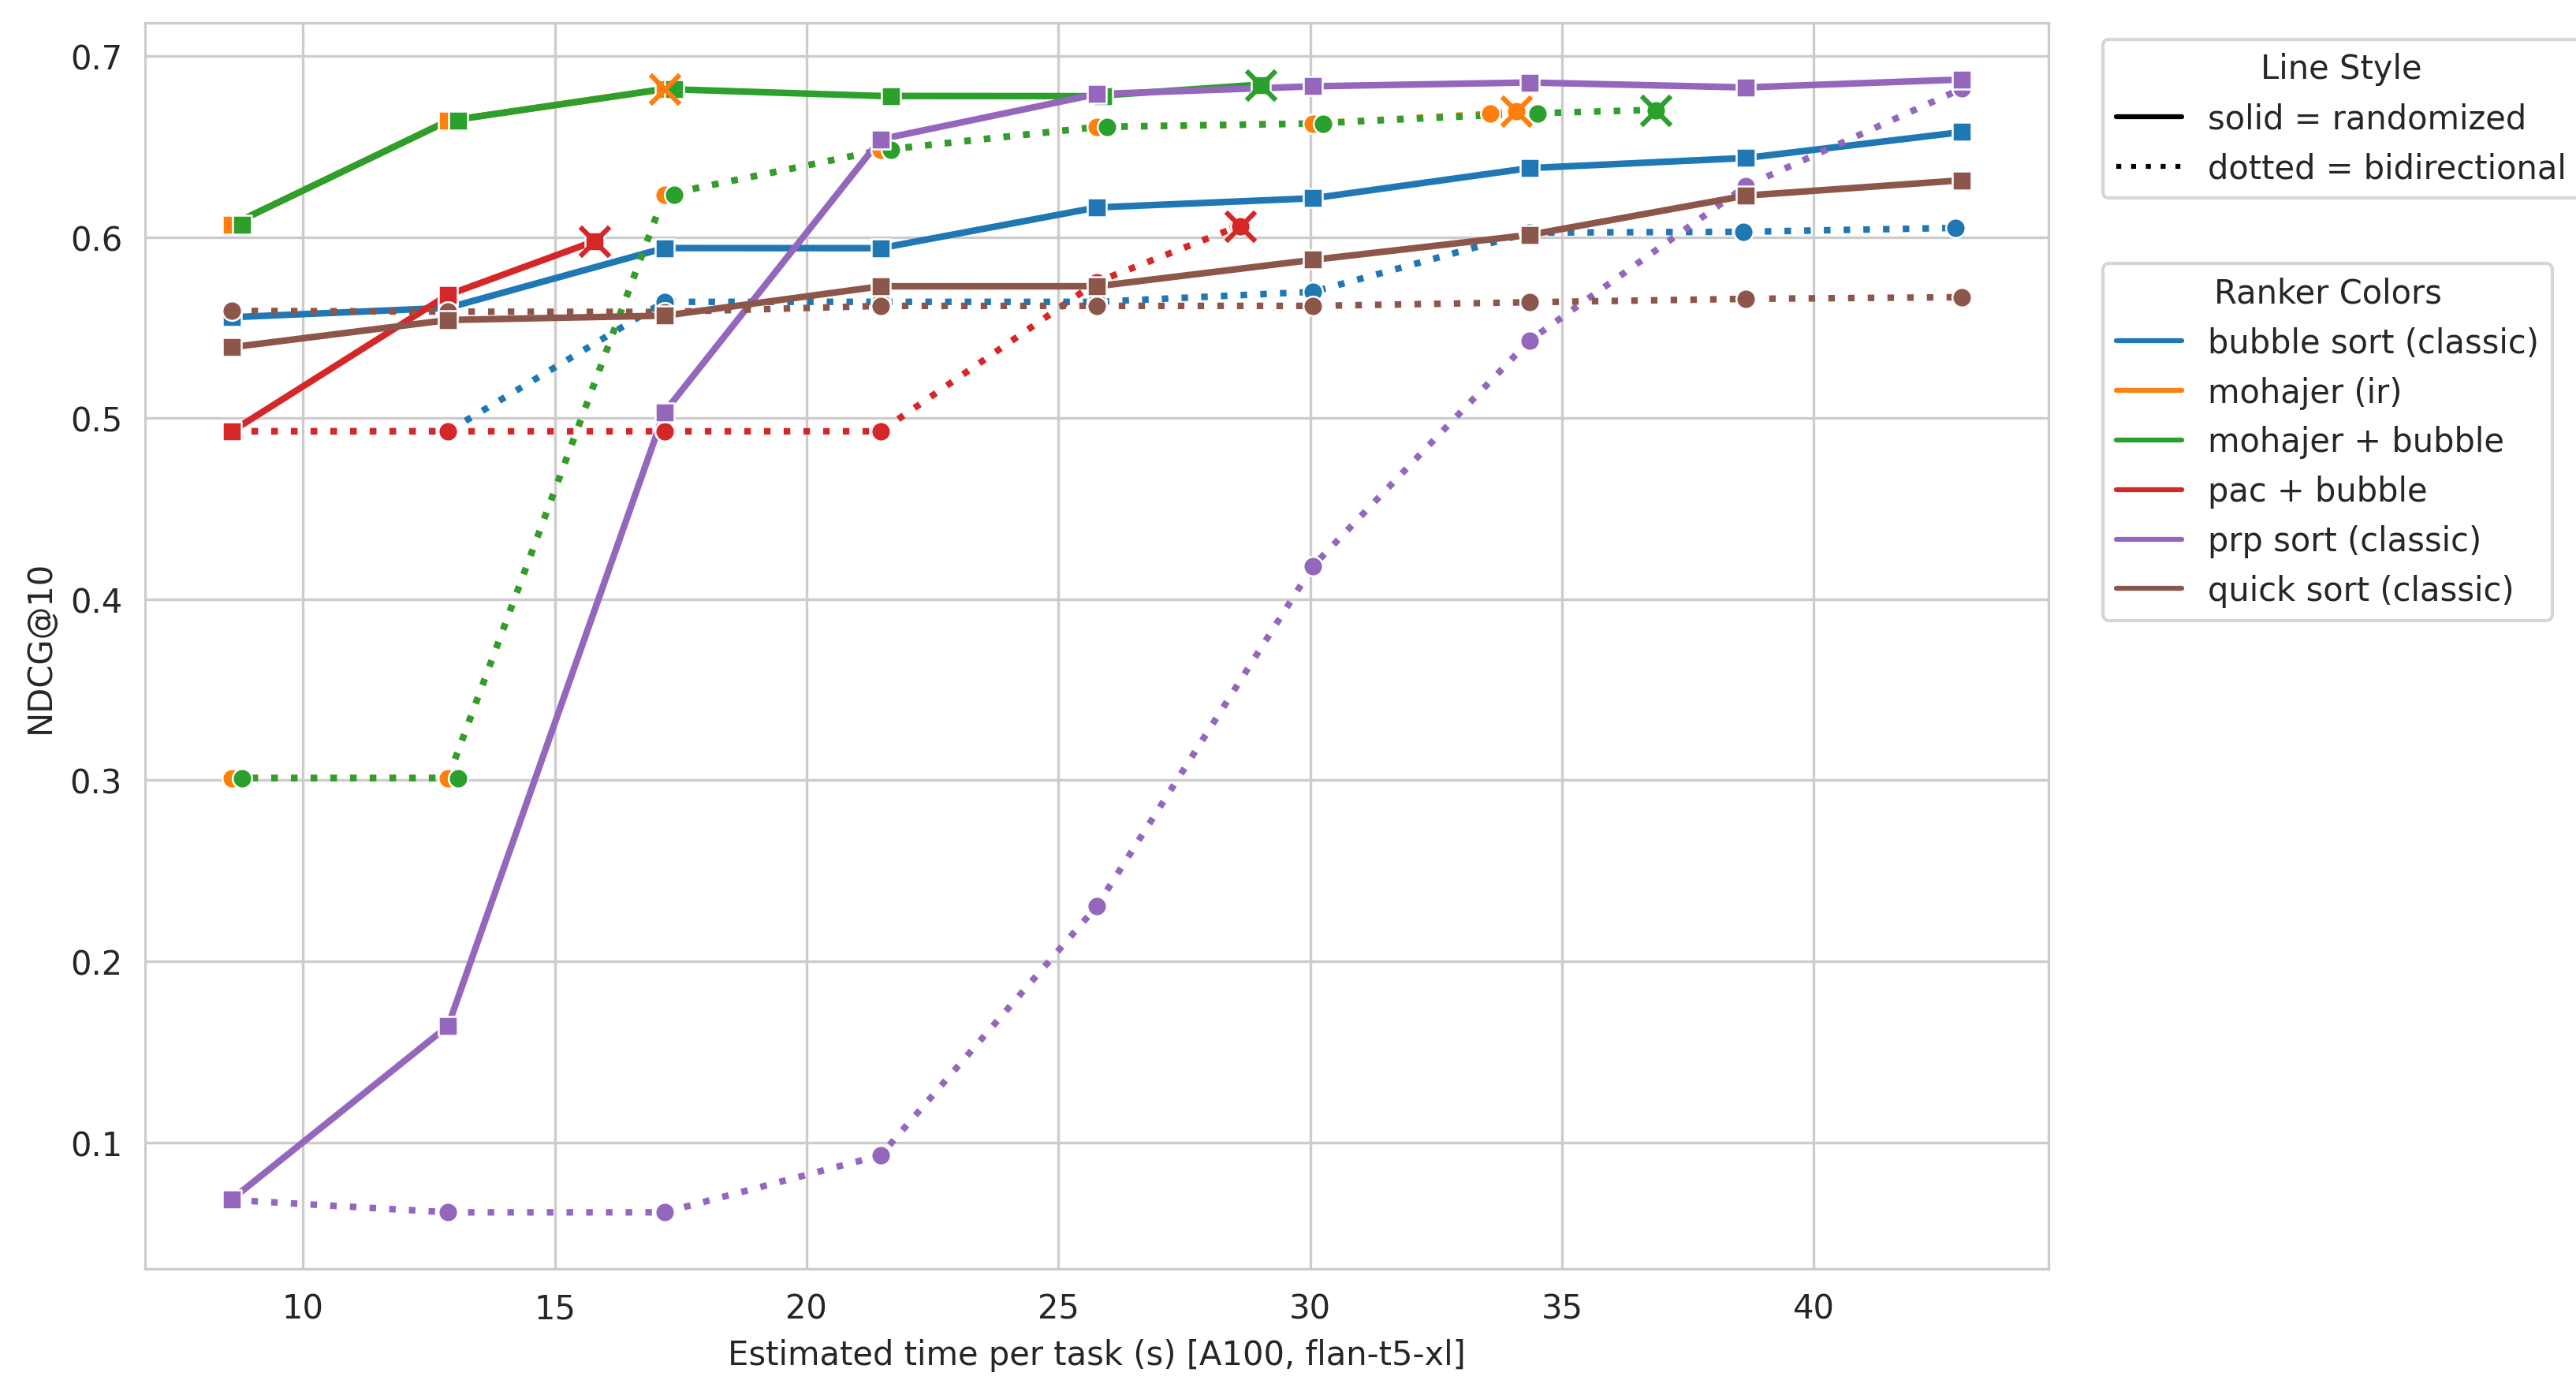
\includegraphics[width=\linewidth,height=0.23\textheight,keepaspectratio]{reports/figures/limit_comparisons_time/limit_comparisons_time_all_flan_a100_both.png}
        \caption{A100}
    \end{subfigure}\hfill
    \begin{subfigure}[t]{0.48\linewidth}
        \centering
        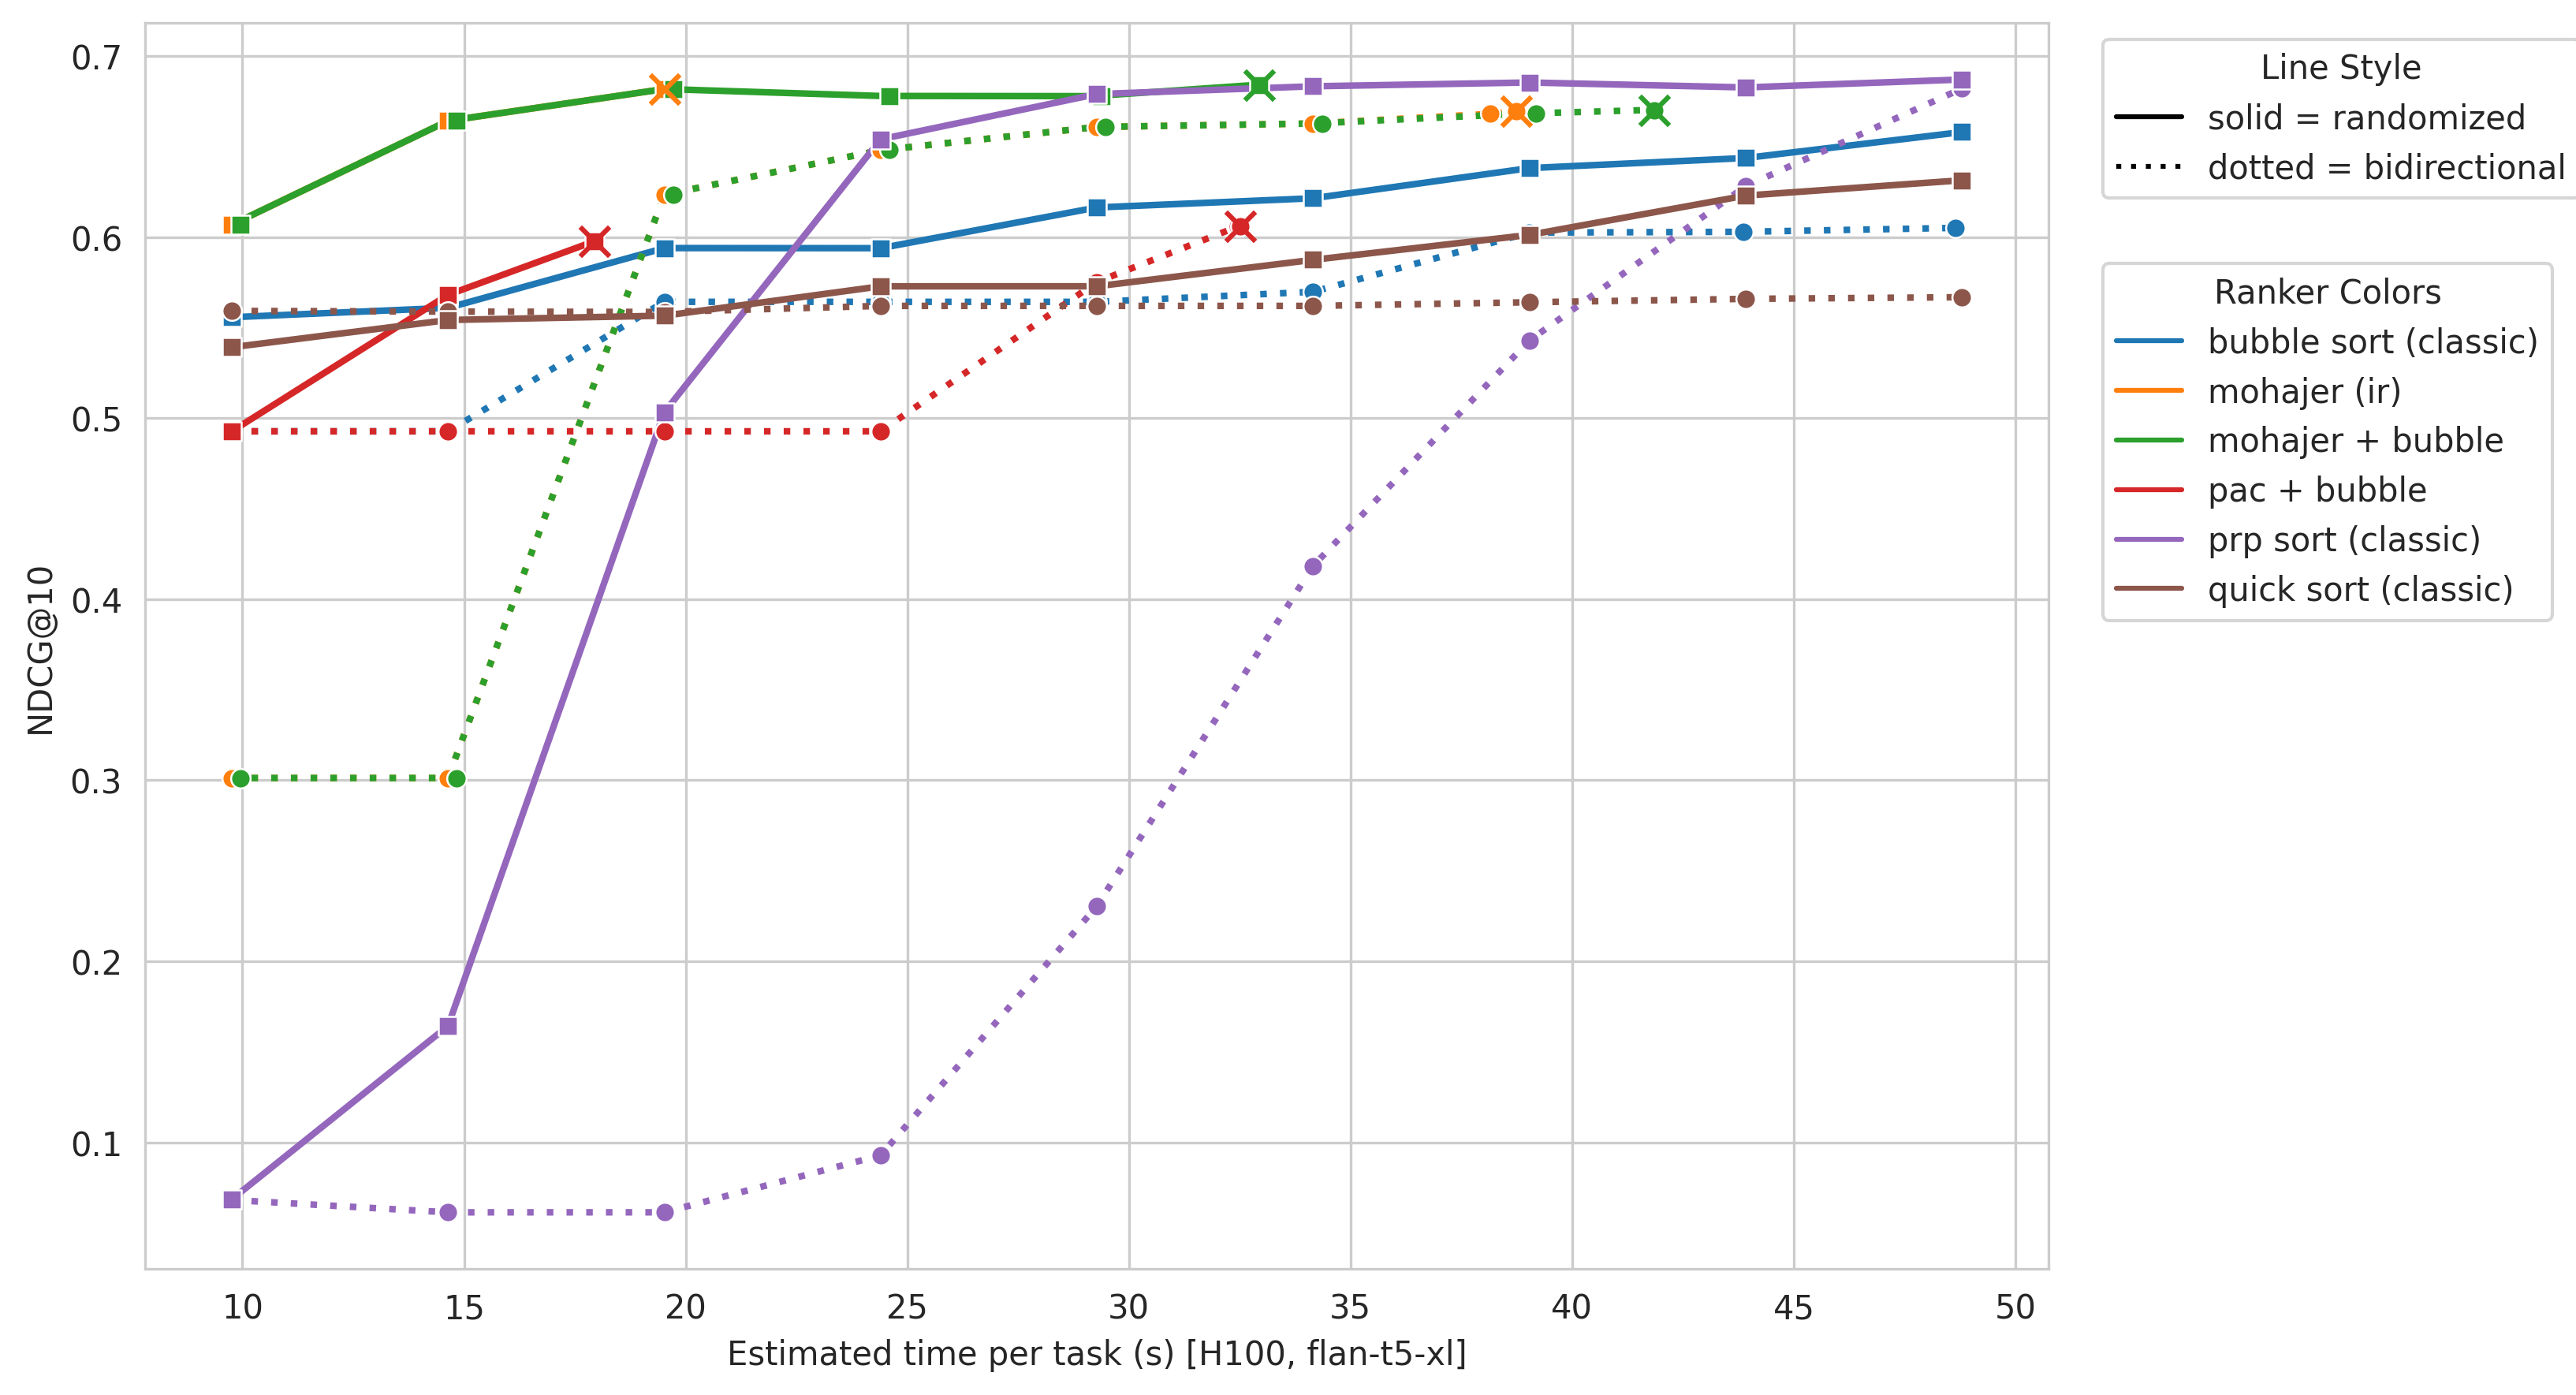
\includegraphics[width=\linewidth,height=0.23\textheight,keepaspectratio]{reports/figures/limit_comparisons_time/limit_comparisons_time_all_flan_h100_both.png}
        \caption{H100}
    \end{subfigure}\hfill
    \vspace{0.2em}
    \begin{subfigure}[t]{0.48\linewidth}
        \centering
        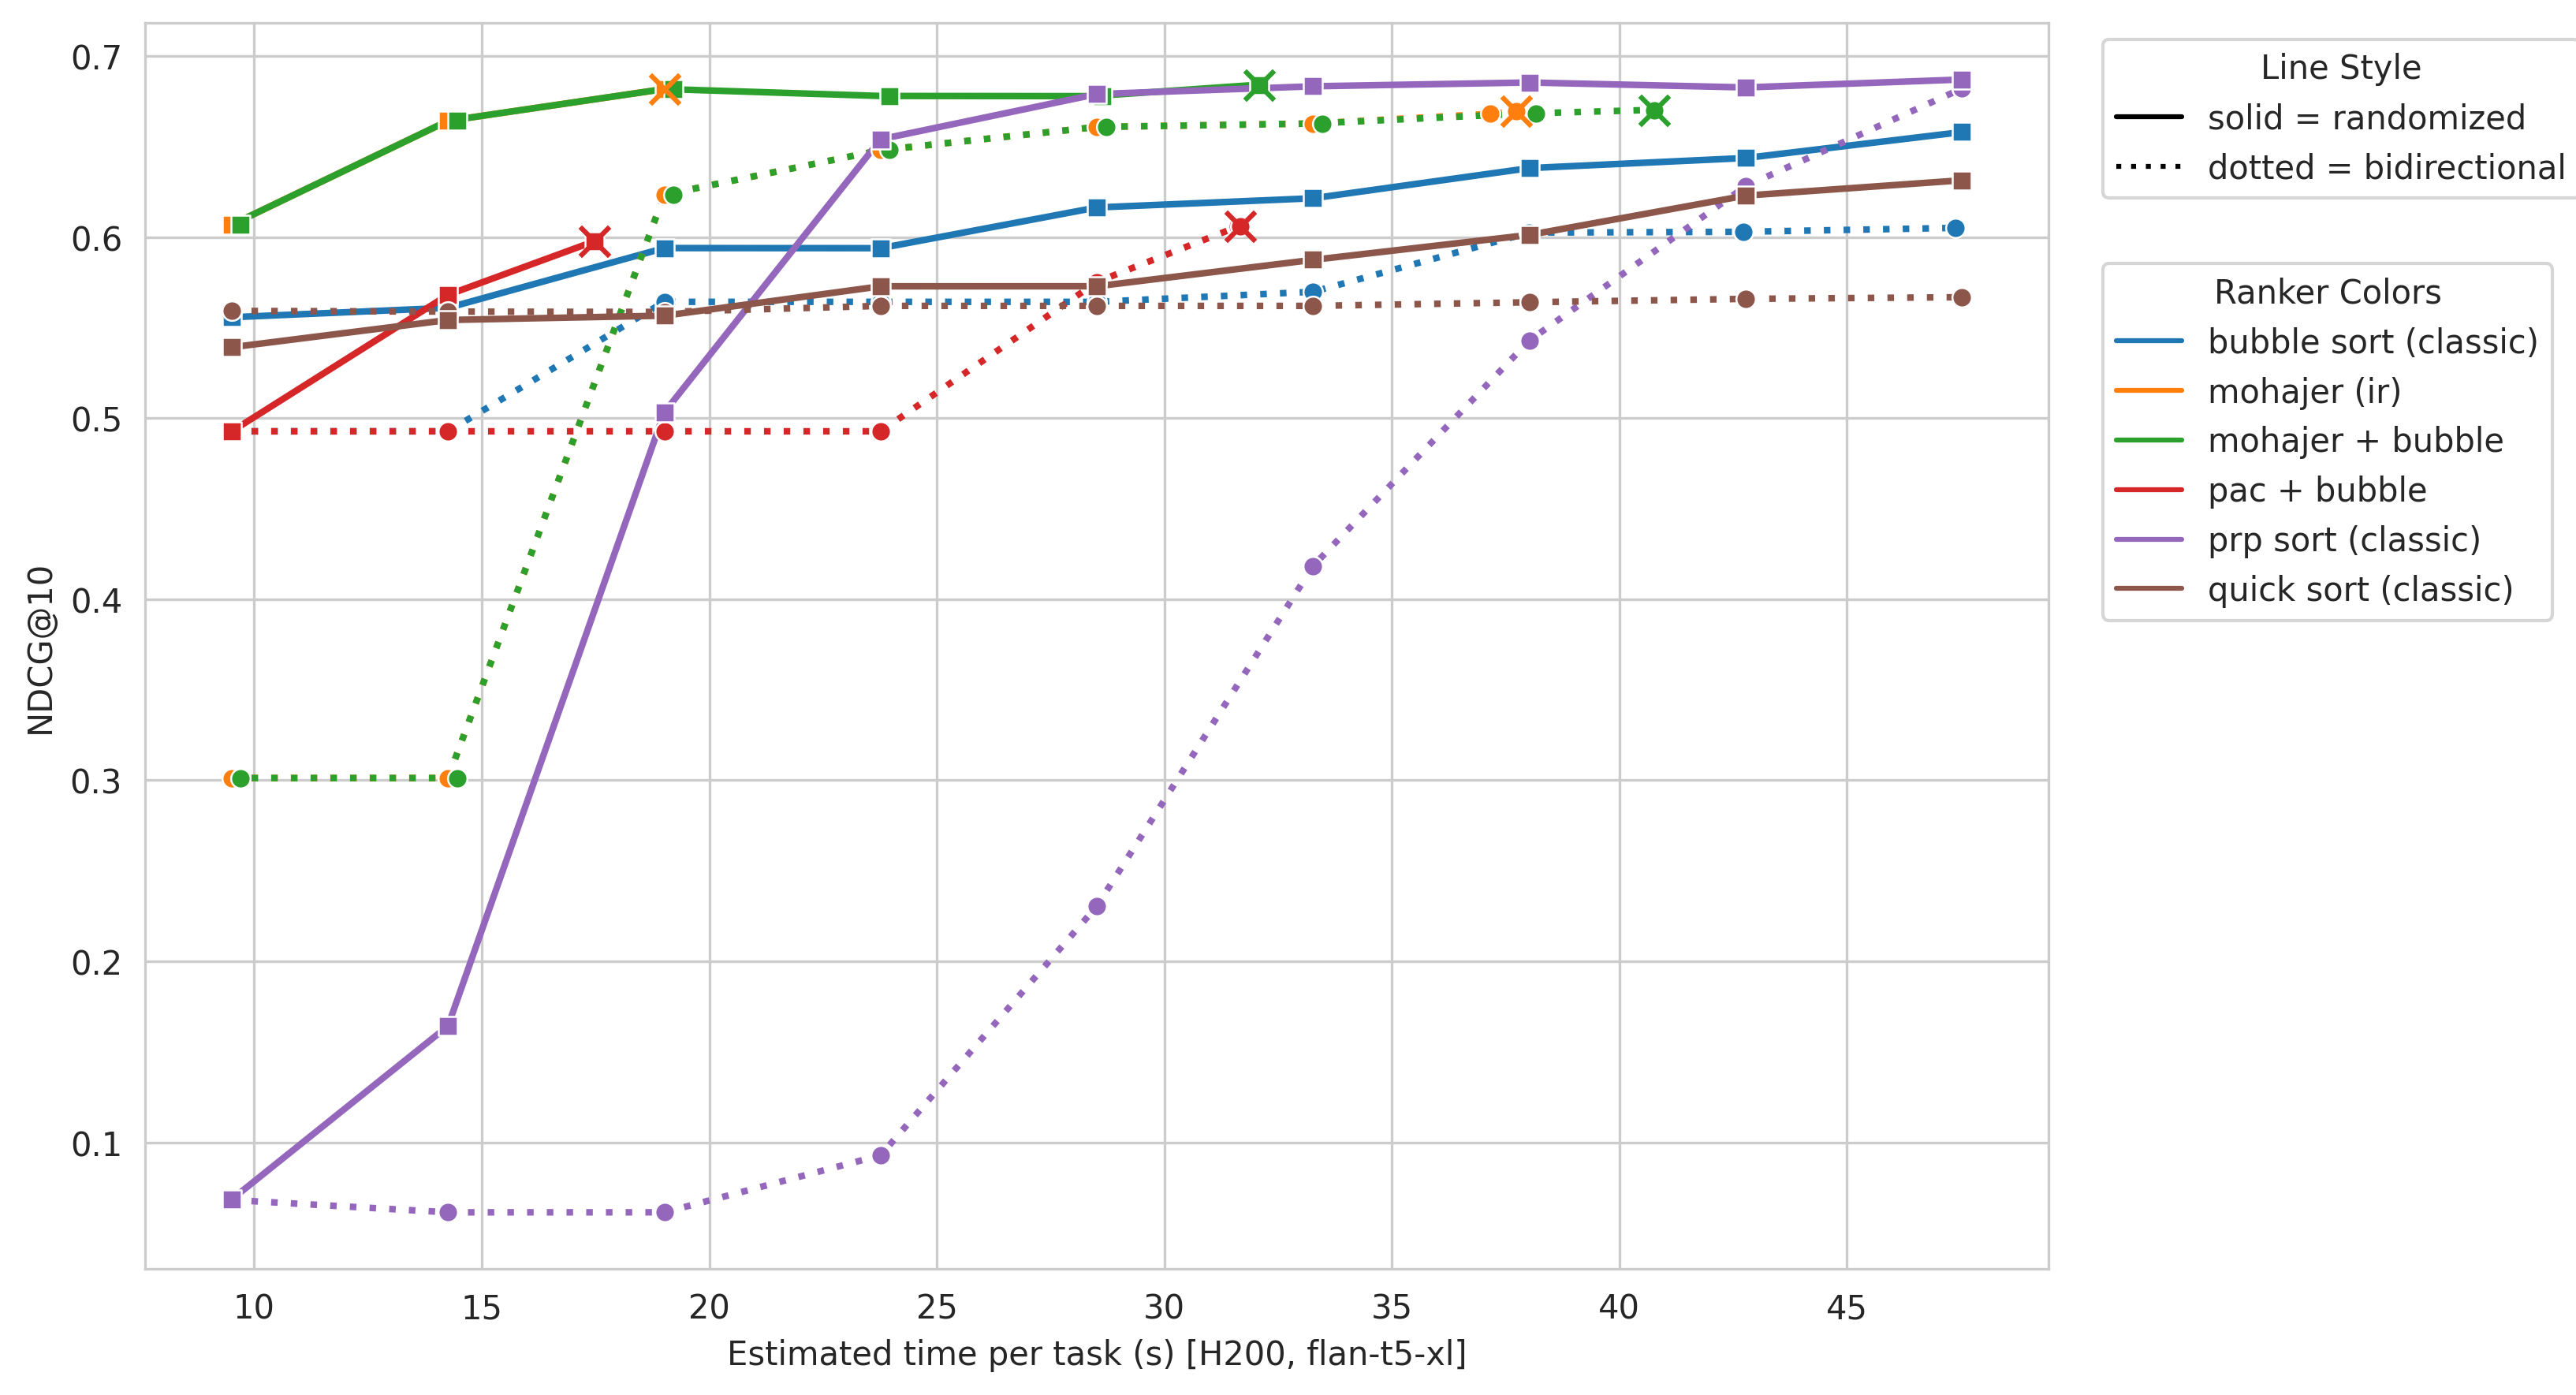
\includegraphics[width=\linewidth,height=0.23\textheight,keepaspectratio]{reports/figures/limit_comparisons_time/limit_comparisons_time_all_flan_h200_both.png}
        \caption{H200}
    \end{subfigure}
    \caption{All datasets (Flan-T5-XL): NDCG@10 vs estimated time per task across GPUs, with both oracles shown. Colors denote rankers; solid lines are randomized and dotted lines are bidirectional. Peak markers (X) are shown for Mohajer/PAC variants.}
    \label{fig:limit_time_all_flan_all_gpus}
\end{figure}
\begin{figure}[H]
    \centering
    \begin{subfigure}[t]{0.48\linewidth}
        \centering
        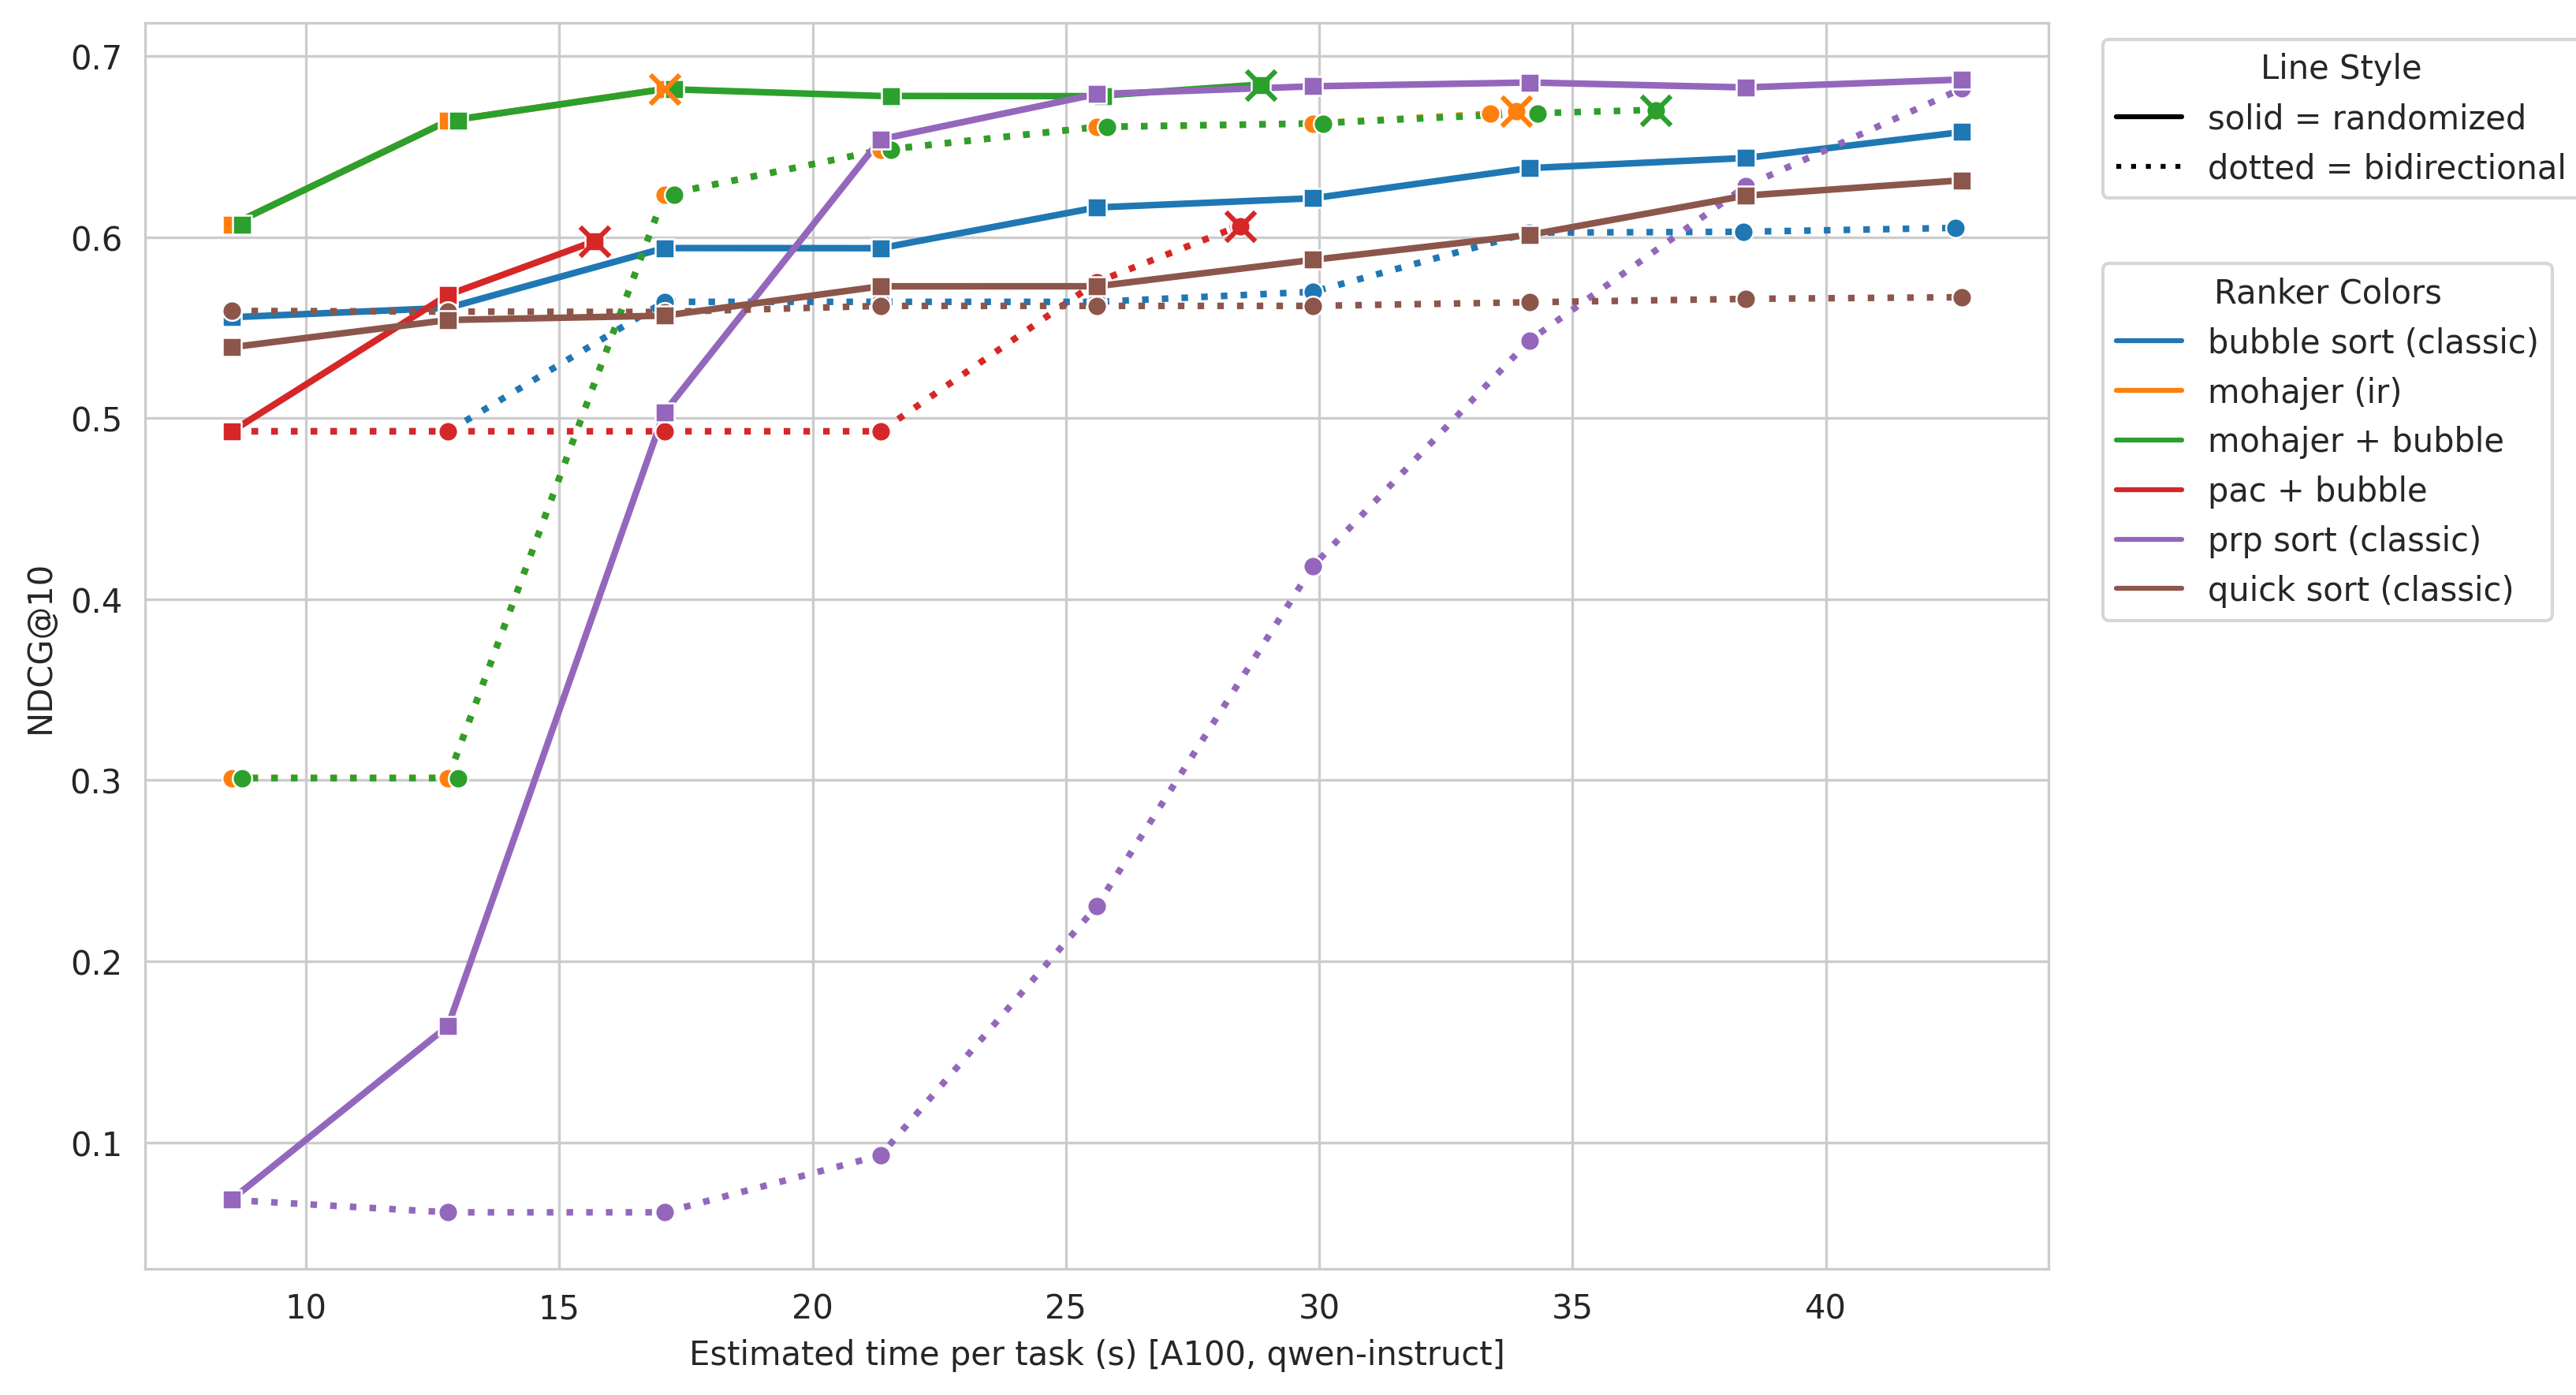
\includegraphics[width=\linewidth,height=0.23\textheight,keepaspectratio]{reports/figures/limit_comparisons_time/limit_comparisons_time_all_qwen_a100_both.png}
        \caption{A100}
    \end{subfigure}\hfill
    \begin{subfigure}[t]{0.48\linewidth}
        \centering
        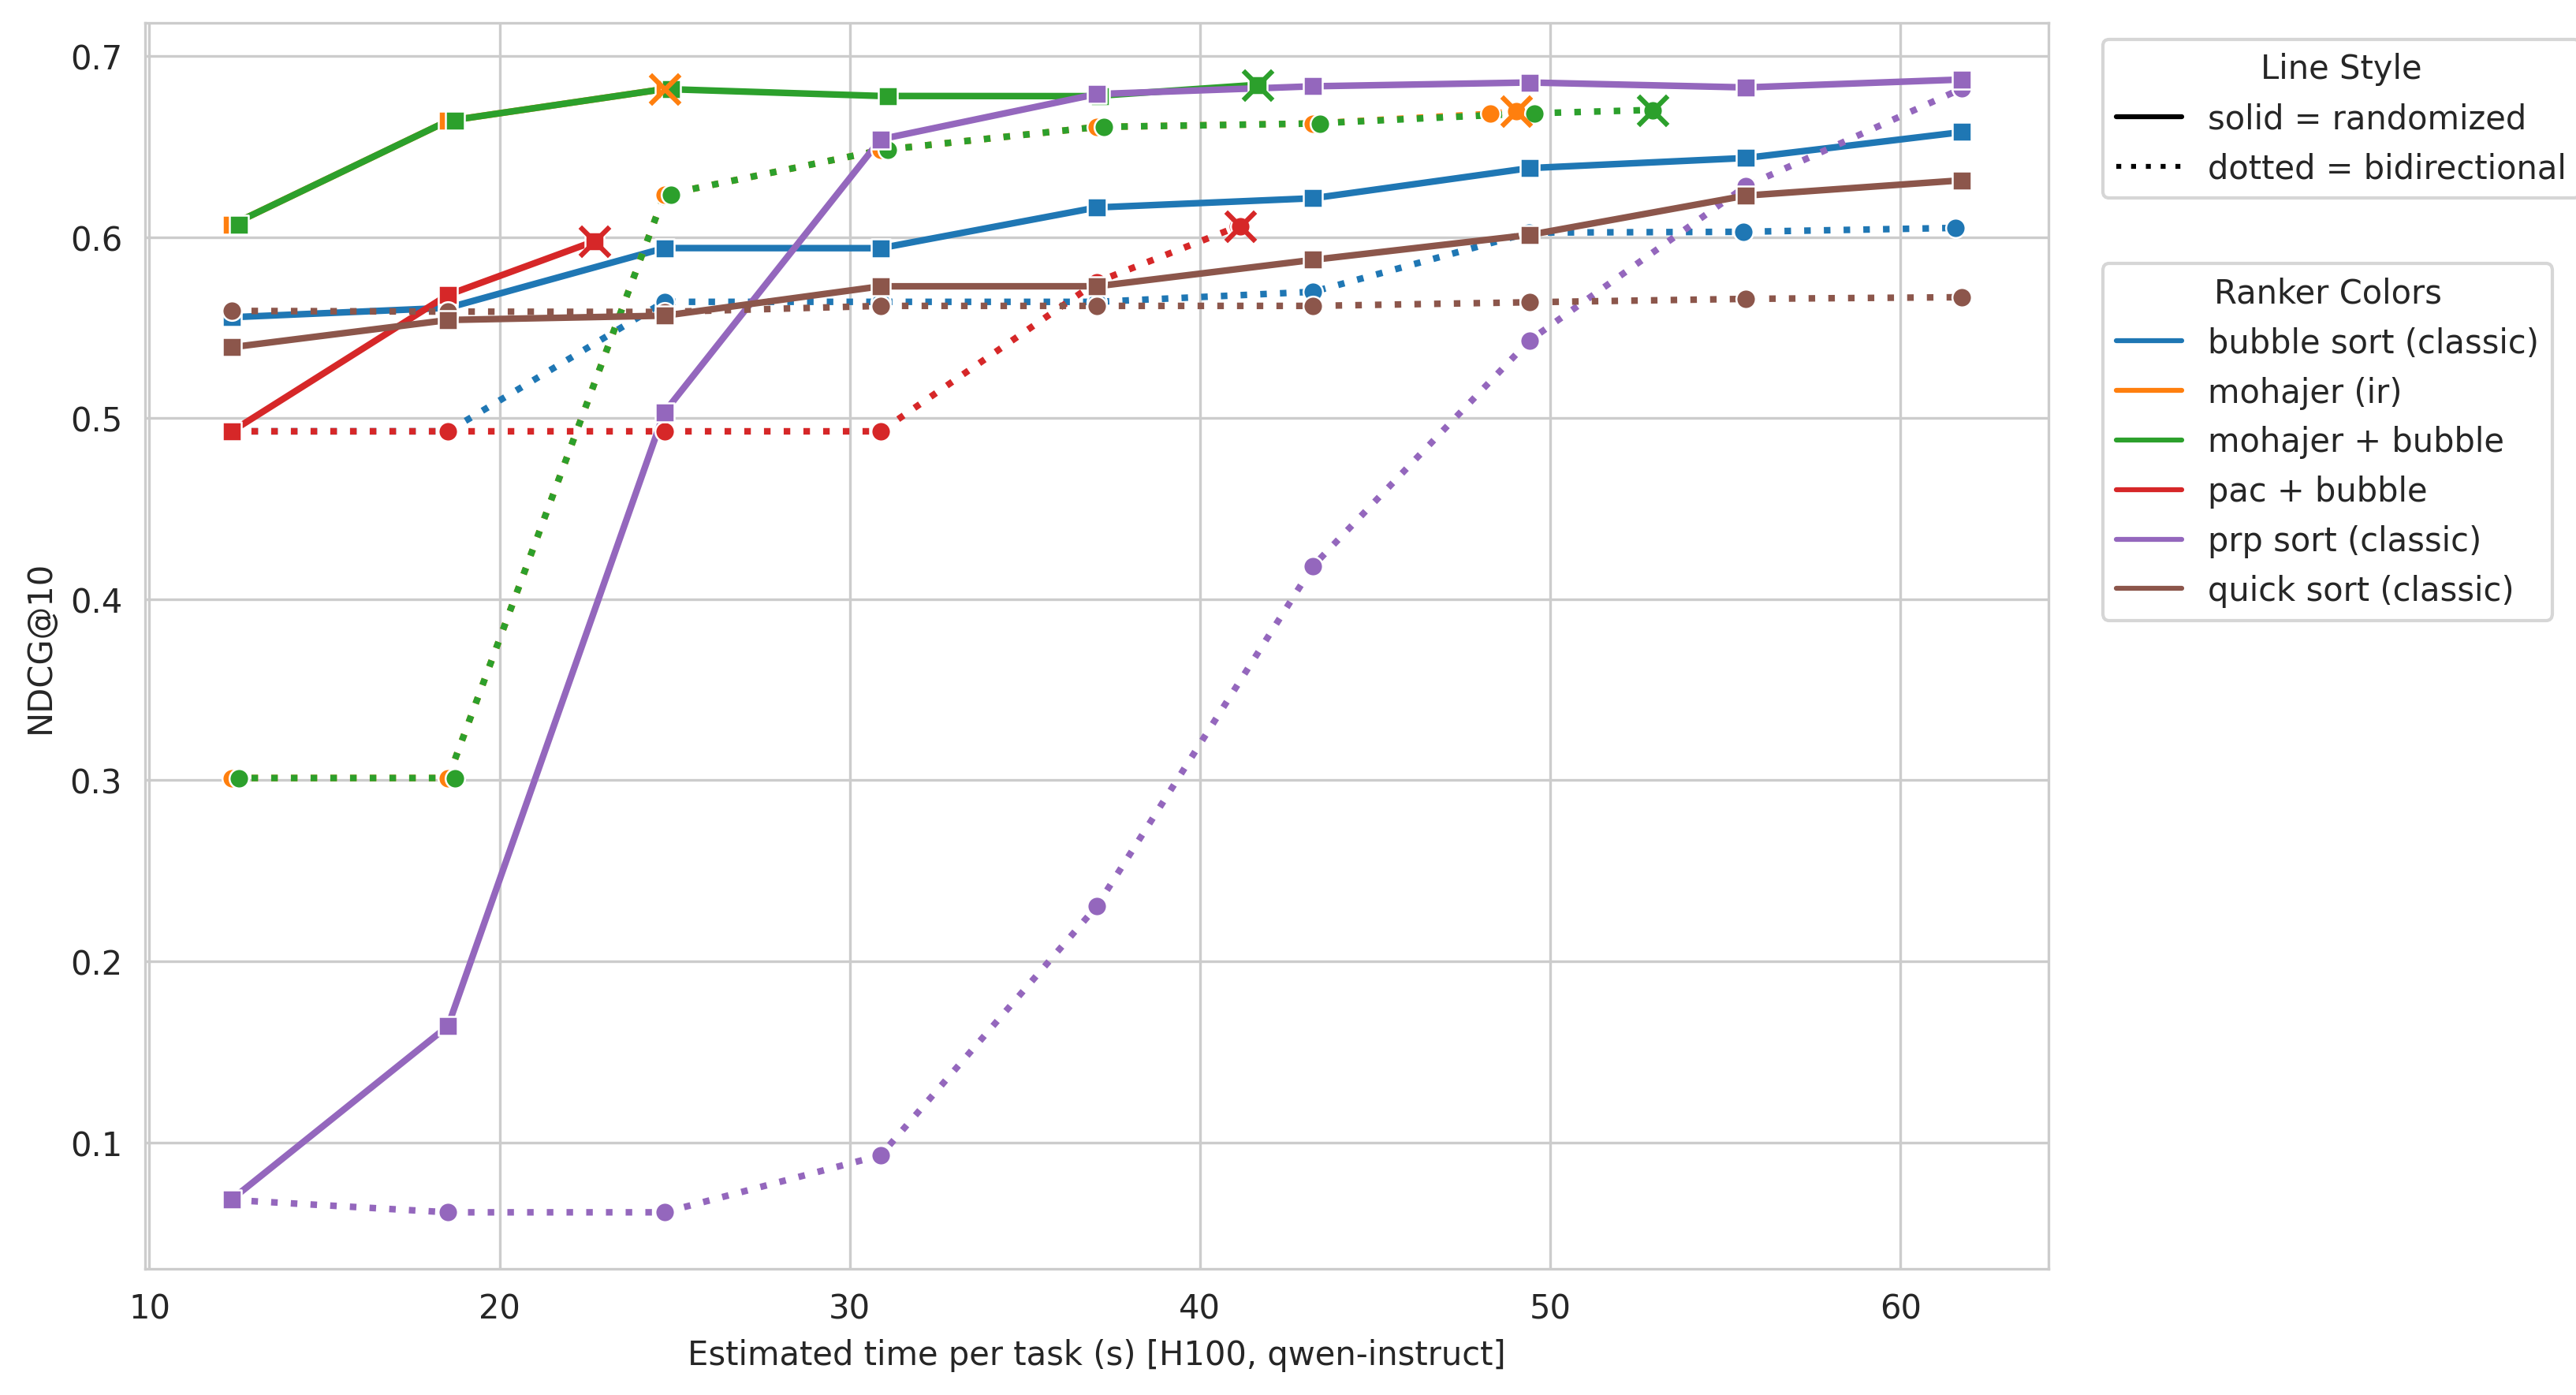
\includegraphics[width=\linewidth,height=0.23\textheight,keepaspectratio]{reports/figures/limit_comparisons_time/limit_comparisons_time_all_qwen_h100_both.png}
        \caption{H100}
    \end{subfigure}\hfill
    \vspace{0.2em}
    \begin{subfigure}[t]{0.48\linewidth}
        \centering
        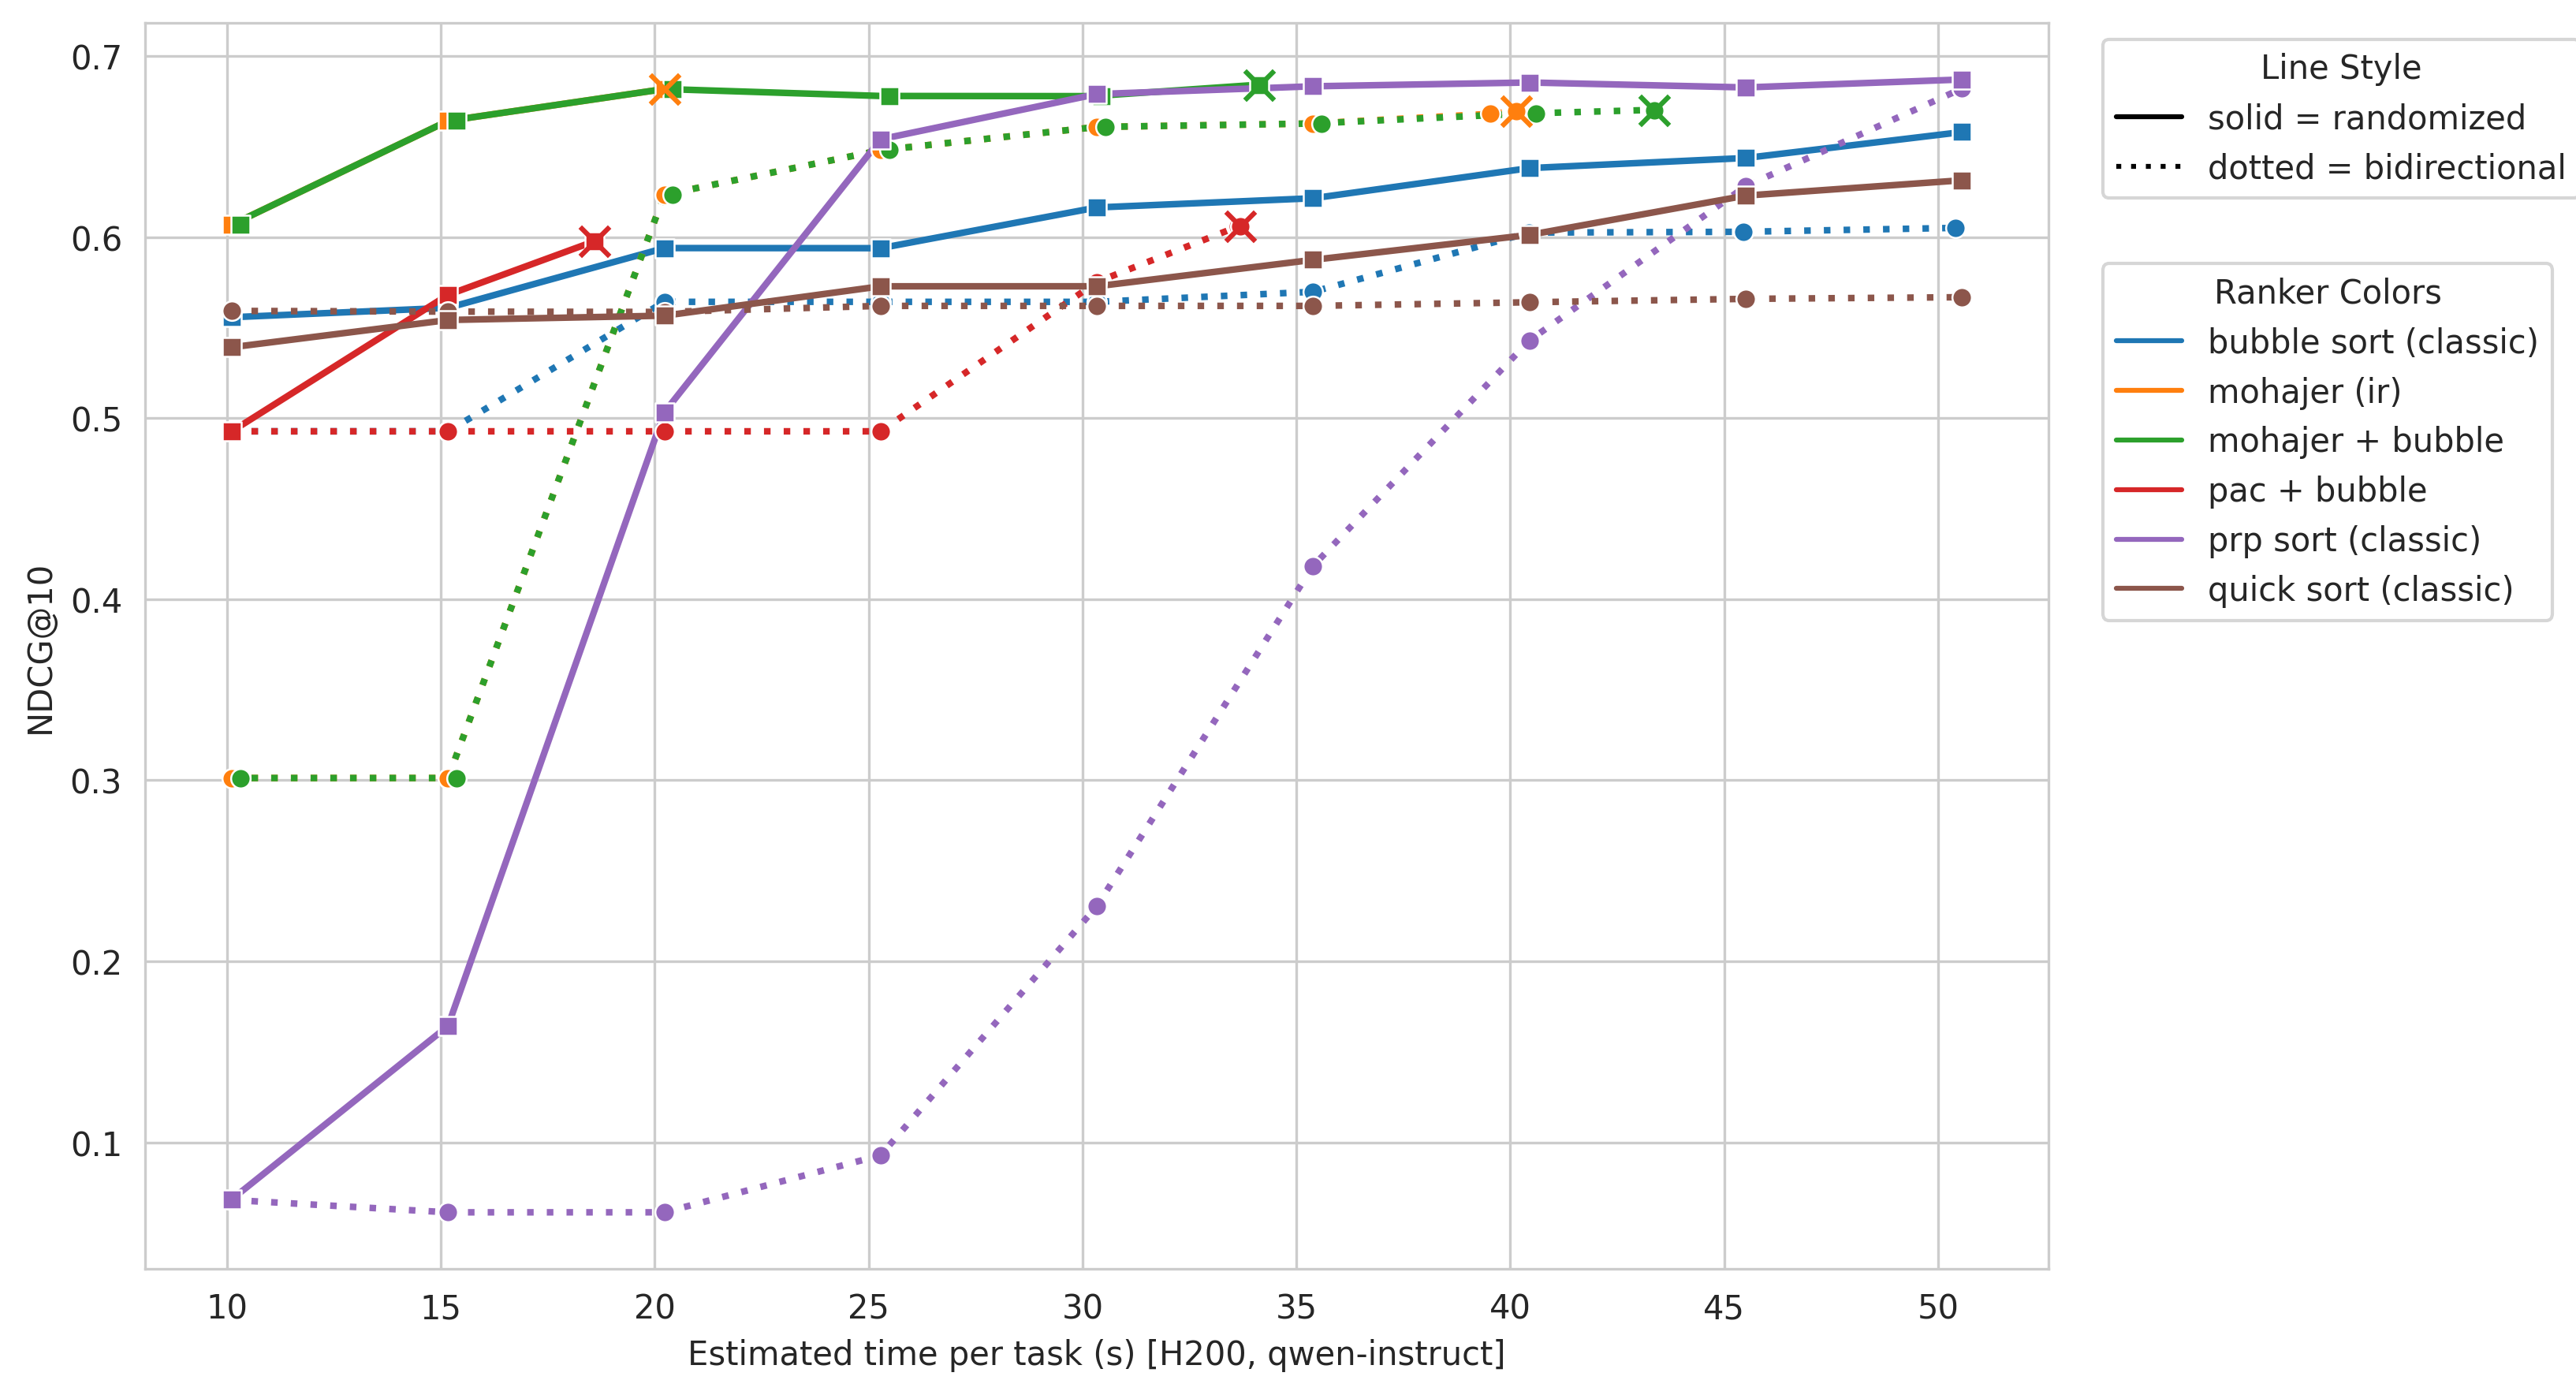
\includegraphics[width=\linewidth,height=0.23\textheight,keepaspectratio]{reports/figures/limit_comparisons_time/limit_comparisons_time_all_qwen_h200_both.png}
        \caption{H200}
    \end{subfigure}
    \caption{All datasets (Qwen-Instruct): NDCG@10 vs estimated time per task across GPUs, with both oracles shown. Colors denote rankers; solid lines are randomized and dotted lines are bidirectional. Peak markers (X) are shown for Mohajer/PAC variants.}
    \label{fig:limit_time_all_qwen_all_gpus}
\end{figure}
\FloatBarrier
\endgroup

% ------------------------------------------------------------
% Parallelization Opportunities
% ------------------------------------------------------------
\section{Parallelization Opportunities}
\label{sec:parallelization}

Both our proposed active ranking algorithms exhibit substantial parallelization potential that could significantly reduce wall-clock latency in practice.

\paragraph{Mohajer.}
The Mohajer algorithm's structure naturally lends itself to parallel execution at all levels.
First, the $K$ independent tournaments used for champion selection can be executed concurrently, as each tournament operates on a disjoint subset of candidates with no inter-group dependencies.
Second, the heapify operation itself is amenable to parallel construction techniques, allowing the initial heap formation to proceed in $O(\log n)$ depth rather than sequential $O(n)$ time.
Finally, within each tournament, pairwise comparisons at the same tree depth are independent and can be batched for simultaneous LLM inference.

\paragraph{Optimized PAC.}
Our optimized PAC algorithm also presents parallelization opportunities, where comparisons of candidates against the selected anchors are entirely independent.
With $K/2$ anchors and a candidate pool of size $K \times \text{pool\_mult}$, these $O(K^2)$ comparisons can be executed in parallel, subject only to the LLM inference throughput.
The subsequent winner-set construction and greedy accumulation require only lightweight aggregation, which remains negligible compared to comparison costs.

\paragraph{Latency implications.}
Assuming an LLM inference API with high throughput (e.g., batched GPU inference or distributed serving), parallelization could theoretically reduce Mohajer's latency from $O(n \log K)$ sequential comparisons to $O(\log Q \cdot \log K)$ parallel rounds, and PAC's latency from $O(K \sqrt{n})$ comparisons to $O(\sqrt{n})$ rounds with batch size $K$.
In our TREC DL experiments, where Mohajer performs $\sim$350 comparisons and PAC $\sim$185 comparisons, parallelization with batch size 10 could reduce round counts to $\sim$35 and $\sim$19 respectively, yielding substantial speedups on systems where comparison latency dominates over LLM throughput.

\end{document}
